
\chapter{Exemplary Application using the Proposed Data Structure}   \label{sec:Example}
\section{Introduction}
    The practical use and the individual steps in the implementation of the proposed data structure are shown by means of an example. In order to represent a real plant a \textit{Teaching Factory} is used. The aim of this plant is to get familiar with automation technology with the help of a PLC and its programming. The plant is modular in order to provide individual stations with defined learning goals, varying from basic topics like digital and analog signals to also more complex tasks like motor control and serial communication. Furthermore, human interaction and safety are included learning contents. An overview of the whole plant is shown in \autoref{fig:TeachingFactory}.
%    \begin{description}
%        \item Separation: The sub-module separation covers the area of digital signals. This task involves the controlled positioning of containers from the input storage area onto the conveyor belt.  
%        \item Filling: In this module, the containers are moved along a conveyor belt and in this process the control of a DC motor can be developed. A dosing unit with stoppers on the conveyor belt and sensors is located at three defined positions along the belt. At these three points the containers can be filled with different or the same granulate. On these three locations the containers can be filled with different or the same granulate. At the end of the conveyor belt, the containers are picked up by the next station. 
%        \item Carthesian Gripper: The gripper is responsible for the further transport of the containers and picks them up from the end of the conveyor belt. Here, the main topic of motor control is further investigated. For example, the origin of each axis must be determined in order to ensure that the containers are placed in the exact position. 
%        \item Load cell: After filling, the weight and thus the filling level of the containers is measured. For this purpose, the container are placed by the gripper on a load cell. After that the load cell transmits the measured value to the PLC via a serial interface. Accordingly, the learning objective in this case is serial communication.
%        \item Thermal processing: After the filling level has been determined, heat treatment of the containers is simulated. This is done by activating a heater via an analog signal and controlling the temperature to a defined value. This task includes the learning objective of analog signals and applied control engineering.  
%        \item Container identification: The containers can be uniquely identified via RFID tags. These tags are attached to the bottom of the containers and have a unique serial number. This module covers the learning goal of component identification and serial communication with the reader of the RFID system. 
%        \item Output storage: This storage area is the final stage of the process. Here the user can take out the filled containers. This station does not offer any specific learning objectives.
%    \end{description}

	\begin{figure}[htp]
		\centering
		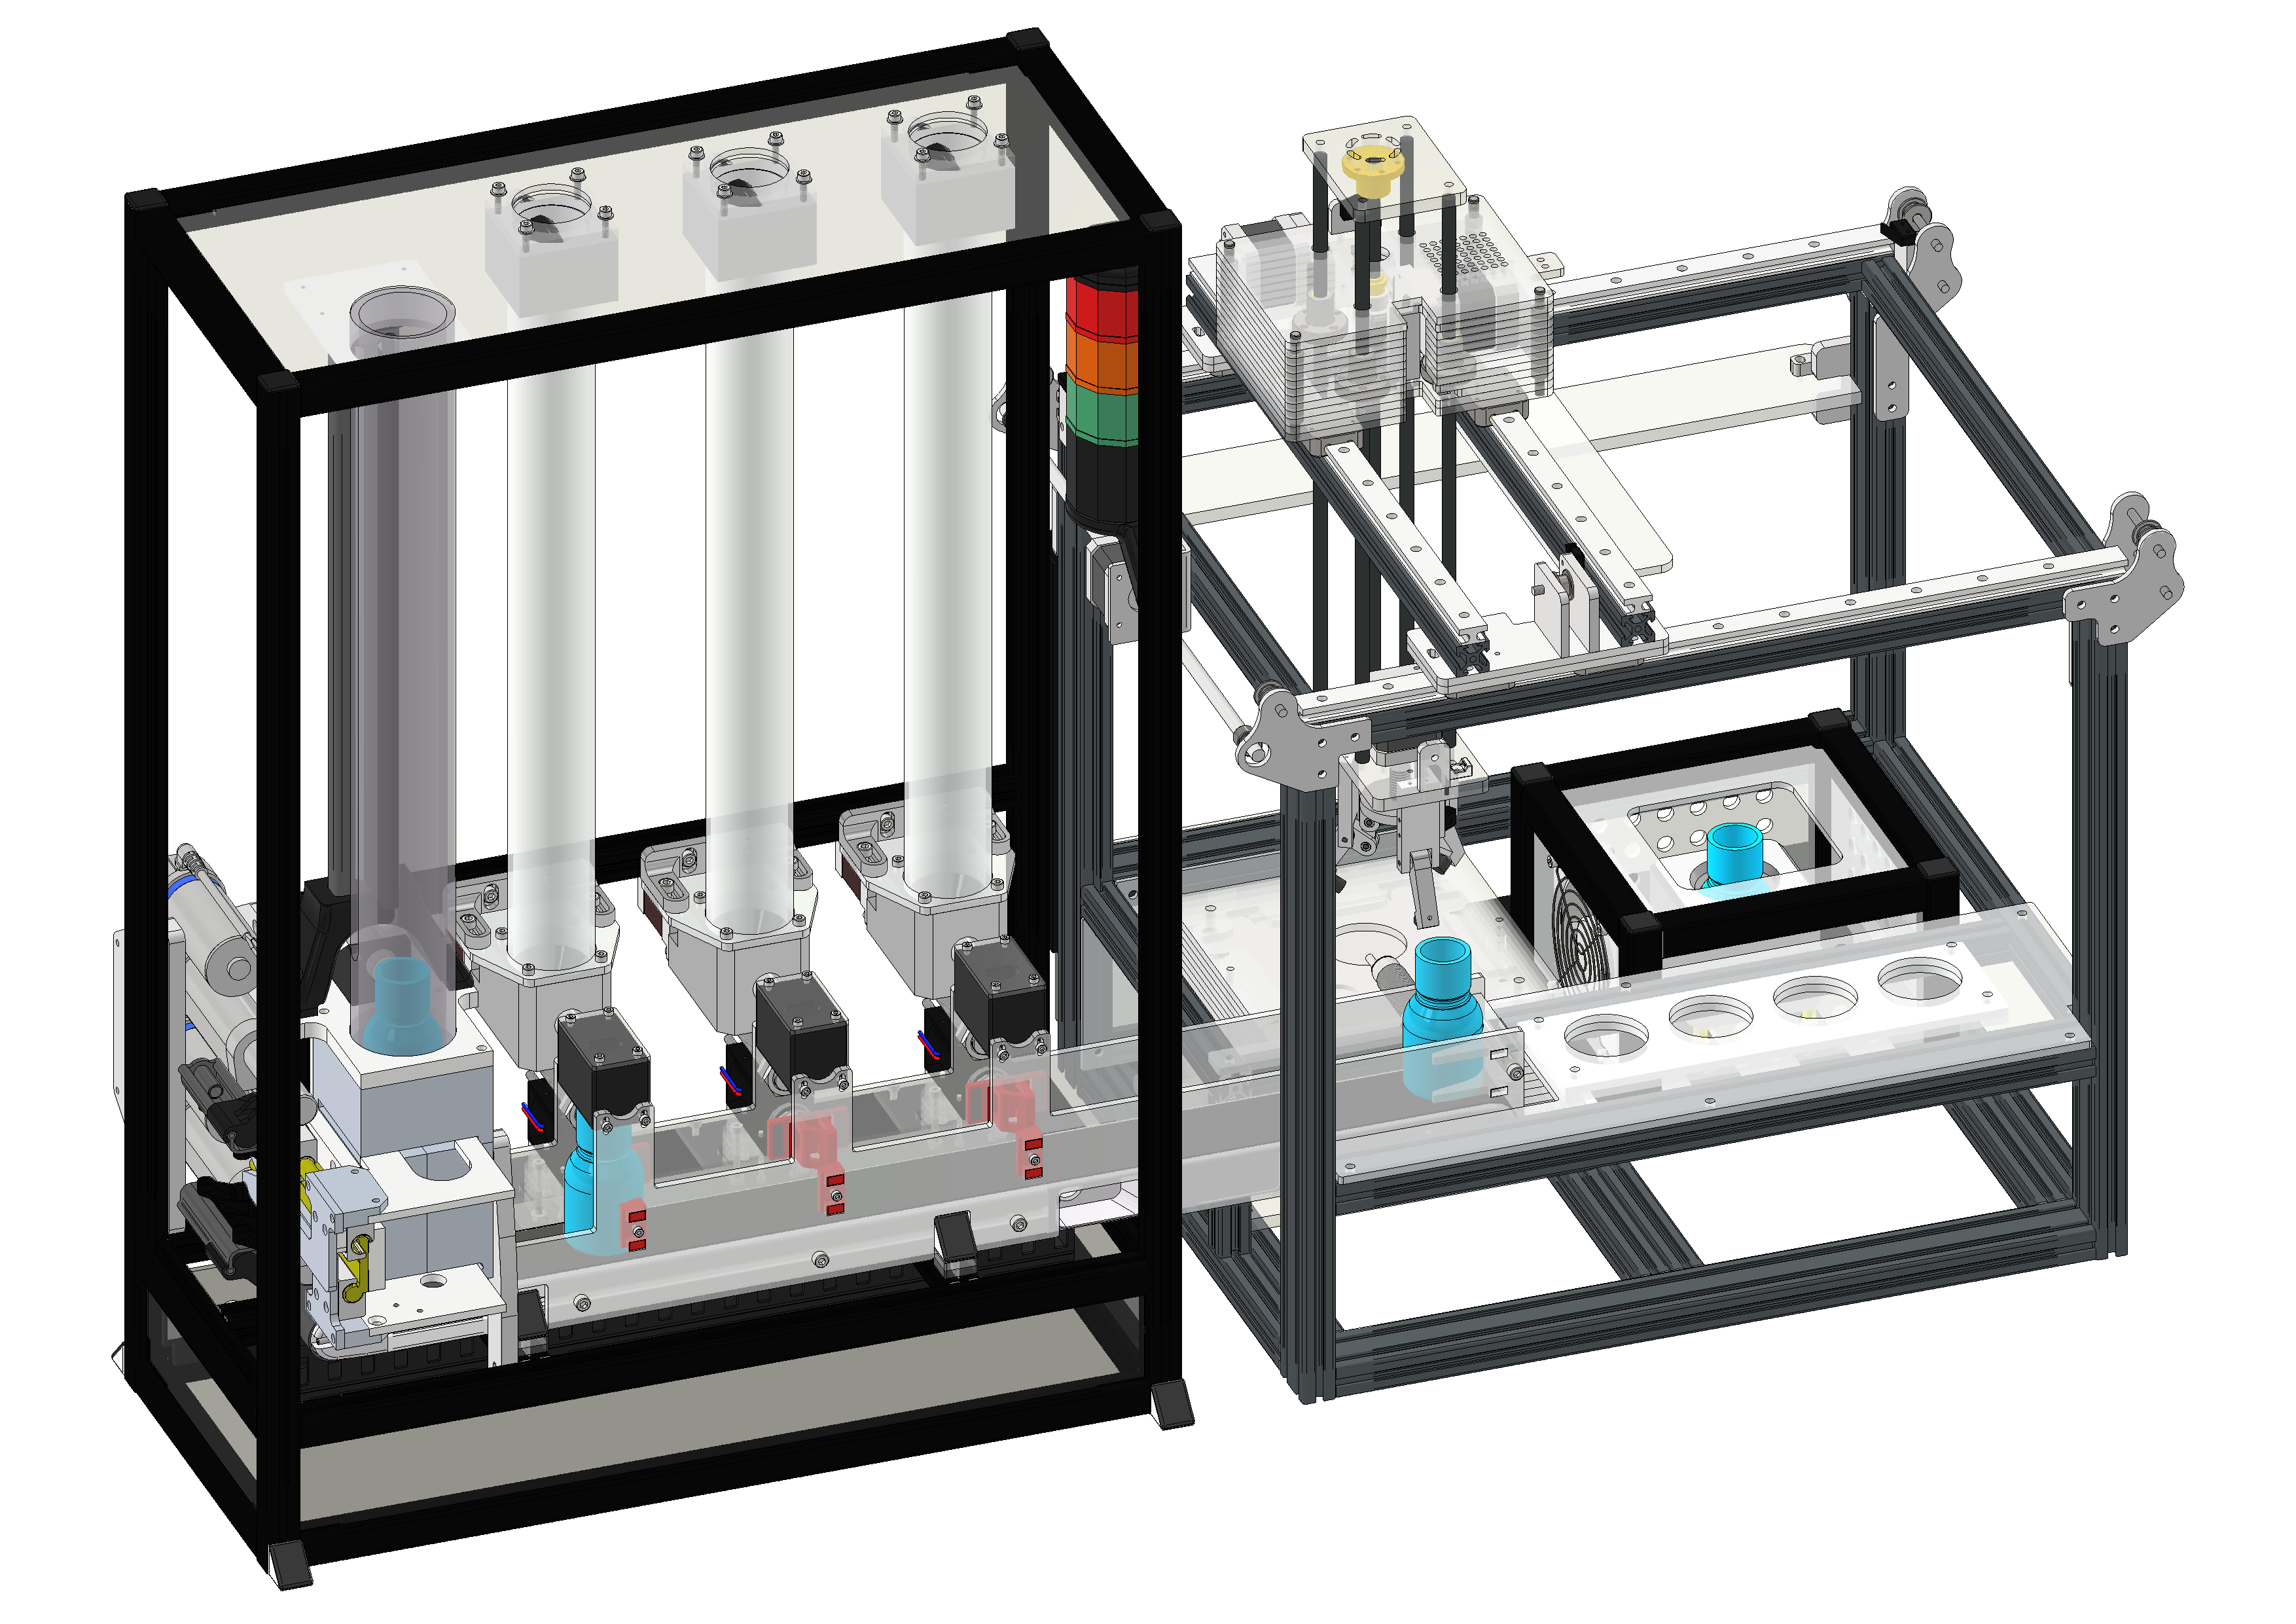
\includegraphics[trim=20mm 0mm 20mm 0mm, clip, width=0.8\linewidth]{figures/TeachingFactory_Real.pdf}
		\caption[The used \textit{Teaching Factory}.]{The used \textit{Teaching Factory}. On the left is the module \textit{Separation} followed by the \textit{Conveyor Belt} with three \textit{Dosing Units}. The right half contains the \textit{Cartesian Gripper} with a \textit{Load Cell} (left), \textit{Thermal Processing} (rear right) and an output storage (front right). For a better overview, further attachments and covers are hidden in this picture.}
		\label{fig:TeachingFactory}
	\end{figure}
	
	

	
\subsection{Module \textit{Separation}}
    % Was macht es 
    The first module offers a fast introduction to the programming of a PLC. Here, the first contact with a PLC can be made and at the same time digital signals for input and output can be used. The task in relation to the \textit{Teaching Factory} is the separation of container from an input storage to the following conveyor belt. The mechanical design of this module is vertically oriented and consists of the input storage in the upper area and the separation in the lower area. The mechanical layout of the module and relevant components for the control are shown in \autoref{fig:ModuleSeperation}.\\
   
    % Signale
    On each of the lower three storage positions a capacitive proximity sensor with a digital output is located. This sensor can be used to detect a container on the corresponding position, where in this case the output signal is set. Above and below the lowest position is a piston attached, which is needed for the actual process of separation. These pistons are moved by a linear motor and controlled by a digital retract or extend signal. In the extended state, the containers can pass the piston undisturbed, while in the retracted state they are stopped at the piston. \\
	\begin{figure}[htp]
		\centering
		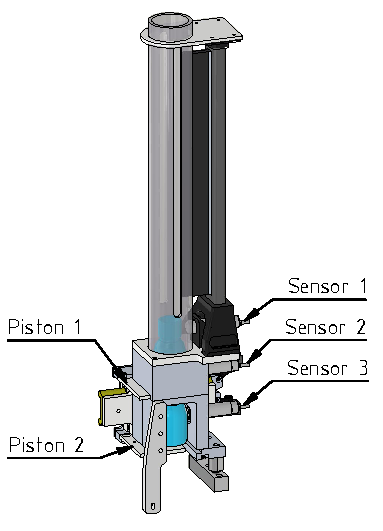
\includegraphics{figures/CadSeperation.pdf}	
		\caption[Overview module \textit{Separation}.]{Overview module \textit{Separation} with the three proximity sensors and the two pistons realizing the separation process.}
		\label{fig:ModuleSeperation}
	\end{figure}
	
\subsection{Module \textit{Conveyor Belt}}
    %This module is the user's first introduction to the control of electrical drives. In order to provide a quick and easy introduction, a DC motor driving a conveyor belt is controlled. In a simplified approach, the velocity of the motor is dependent on the input voltage and the torque is dependent on the current. This allows a relatively easy implementation of a closed loop control and additionally the theoretical aspect of the motor control becomes simple to understand. An encoder is also attached to the motor axis in order to determine the real velocity and position of the motor. Because of this measurement of the position, a servo control of the conveyor belt can be implemented in an additional step.  The difference of a servo control compared to a standard control without encoder is the possibility to move the conveyor belt to an exact position, because the angular position of the motor axis  is known. Furthermore, the encoder provides feedback about the real velocity of the motor and therefore an unwanted stop can be detected immediately. 
     This module is the user's first introduction to the control of electric drives. Using a DC motor with its comparably simple design allows the theoretical background easier to understand and the main focus can lay on the controlling. In addition, an encoder is attached to the motor axis to determine the actual speed and position of the motor. By this measurement of the position, an optional servo control of the conveyor belt can be implemented in a further step and thus enable an exact positioning. Moreover, through the feedback of the actual speed of the motor, an undesired stop can be detected immediately. In a second step, the knowledge of motor control is further expanded with stepper motors. \\

    
 %   The conveyor belt has a total length of \SI{400}{\milli\meter} and is divided into the following sections: Input, Filling (three times) and Output. At the beginning of the belt conveyor, the containers are taken from the station \textit{separation}, where they are placed on the belt. After that, the containers go through three identical possibilities of filling by means of a dosing unit. The dosing units can be filled individually and as a result use the same or a different granulate. To simplify the process of filling a container, a stopper and a proximity sensor are located below each dosing unit. The stopper is similar to those of the station \textit{separation}, but in contrast only one digital signal is needed for controlling, which retracts the slider. If this signal is not set, the slider is extended and the containers are stopped on the conveyor. The proximity sensors are identical to those of the station \textit{separation} and set a digital output signal if a container is detected. This combination of sensors with the stoppers and the conveyor belt allows a container to be placed precisely under a dosing unit. At the end of the conveyor belt, the containers are passed over to the next station. To ensure the transport of the containers to the next station, again a proximity sensor is located at the defined transfer position. 
    The conveyor belt is the main part of the filling process and is divided into three sections: input, filling (three dosing units) and output. At the beginning of the conveyor belt, the containers are passed from module \textit{separation}. After that, the containers go through three identical dosing units used for filling. These dosing units each consist of a helix driven by a stepper motor. In order to simplify the filling process of a container, a stopper and a proximity sensor are located under each dosing unit on the conveyor belt. The stopper normally locks the container and can be retracted via a digital signal. The proximity sensors are identical to those of the module \textit{separation} and provide a digital output signal when a container is detected. This combination of sensors with the stoppers and the conveyor makes it possible to precisely place a container under a dosing unit. At the end of the conveyor belt, the containers are passed on to the next module, where a proximity sensor is also placed at the defined pick-up position. \\
    
    In this example, the user has to create the control of the conveyor belt in the first step. After that, the software is extended with the digital signals of the stoppers and proximity sensors. Finally, the control for the dosing units has to be implemented, where large parts of the control are identical to the conveyor belt. The mechanical layout and relevant components  are shown in \autoref{fig:ModuleFilling}. 
	\begin{figure}[htp]
		\centering
%	    \FramedBox{10cm}{15cm}{Some text}
	    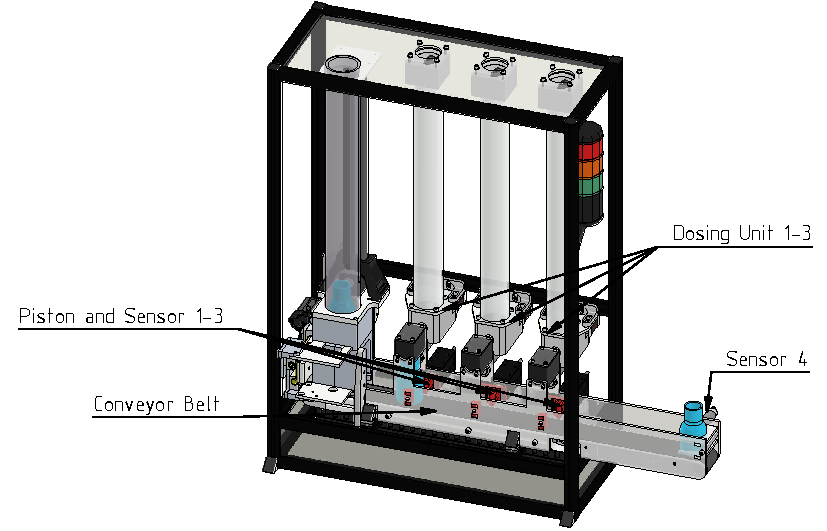
\includegraphics{figures/CadConveyor.pdf}
		\caption[Overview module \textit{Conveyor Belt}.]{Overview module \textit{Conveyor Belt}. On the left side teh module \textit{Separation} is shown. In the middle the conveyor belt is located with the three dosing units for filling. On the right side the pick-up position to the next module is shown at sensor 4.}
		\label{fig:ModuleFilling}
	\end{figure}
    
    
	\subsection{Module \textit{Cartesian Gripper}}
	    In this module, the subject of controlling a stepper motor is further discussed and expanded. Topics such as moving to a specific position and the zero point can be covered in this module. The mechanical layout itself consists of a gripper and three axes for movement in the X, Y and Z direction. The axes are controlled by a stepper motor and have two limit switches for safety purposes. The gripper itself is also driven by a stepper motor including two limit switches. The mechanical layout of the module and relevant components for PLC coding are shown in \autoref{fig:ModuleGripperIntroduction}.\\
	    
	    The \textit{cartesian gripper} is the main component following the filling of the containers and is responsible for the further transport of these to the final modules. Therefore, the gripper has to pick up the containers from the conveyor belt and place them sequentially in the modules \textit{load cell} and \textit{thermal processing}. Finally, the container has to be placed in the output storage. In order to ensure sufficient positioning of the containers in the modules, the PLC controller must be able to position the gripper precisely. A correctly set reference point for each axis is an essential requirement for this.
        	\begin{figure}[htp]
    		\centering
  %  		\FramedBox{10cm}{15cm}{Some text}
            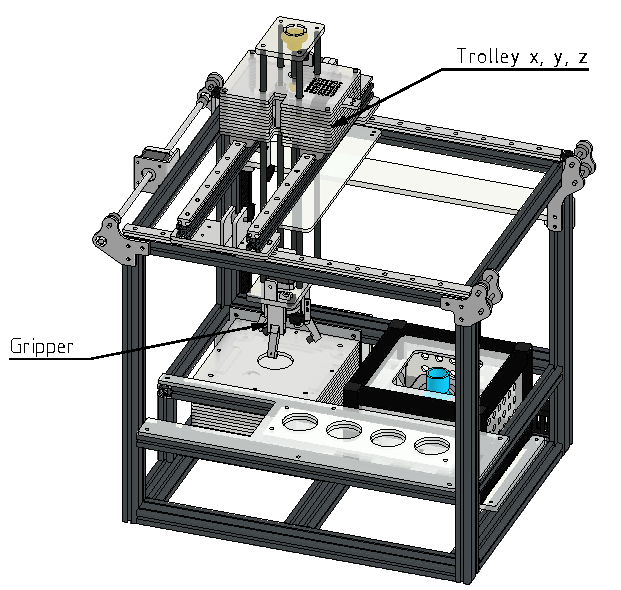
\includegraphics{figures/CadGripper.pdf}
    		\caption[Overview module \textit{Cartesian Gripper}.]{Overview module \textit{Cartesian Gripper} with the following modules and the trolley. In the lower left corner the container are picked up from the conveyor belt.}
    		\label{fig:ModuleGripperIntroduction}
    	\end{figure}
    
	
	\subsection{Module \textit{Load Cell}}
	    % Was soll es machen
	    In this module the filling level of a single container is determined by means of a weight measurement. A laboratory scale is used as load cell, which sends the current measurement result as text via a serial interface and allows the user to get in touch in communication with external devices. As already mentioned, the container positioning is done by the \textit{cartesian gripper}. The layout of this module is shown in \autoref{fig:ModuleLoadCellIntroduction}.\\
	    
	    The task of the user is to establish communication with the load cell via an RS-232 interface. Furthermore, the scale must be calibrated by sending a defined command and the received messages must be interpreted. Only if the filling level is correct, the containers are passed to the module \textit{thermal processing}.
    	\begin{figure}[htp]
    		\centering
    	    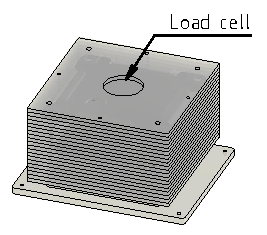
\includegraphics{figures/CadLoad.pdf}
    		\caption[Overview module \textit{Load Cell}.]{Overview module \textit{Load Cell}. The containers are placed in the middle of the platform. }
    		\label{fig:ModuleLoadCellIntroduction}
    	\end{figure}
	
	
	\subsection{Module \textit{Thermal Processing}}
	After checking the filling level, a thermal treatment of the containers is done in this module, using four heating cartridges and two thermocouples. These components are used to raise the temperature of the containers to a defined value. The interface for the heating cartridges and the thermocouples are analog signals and thus the user is able to work on this module at an early stage, although it is the last step in the manufacturing process. The structure and the relevant components are shown in \autoref{fig:ModuleThermalIntroduction}.\\
	
    As mentioned earlier, the task of the user here is to use the analog signals to finally establish a temperature control. In this context, \textit{Timer} components may also be used, for example, to maintain the temperature for a defined period of time.
	\begin{figure}[htp]
		\centering
		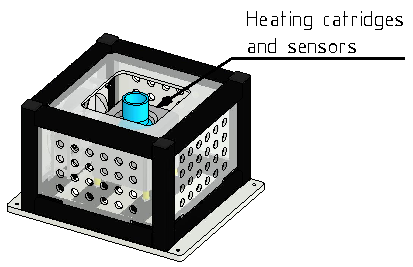
\includegraphics{figures/CadThermal.pdf}
		\caption[Overview module \textit{Thermal Processing}.]{Overview module \textit{Thermal Processing}. The heating cartridges, thermocouples and the container are located in the central block. For safety purpose and in order to cool the block down fans are mounted on the side. }
		\label{fig:ModuleThermalIntroduction}
	\end{figure}
	
	
    \subsection{Setup for Testing}  \label{sec:ExampleSetupTesting}
        % Software
        A list of the used software for this example can be found in \autoref{tab:UsedSoftware}. \\
        \begin{table}[htp]
    	    \footnotesize
    	    \centering
    		\caption{Used software in the example \textit{Teaching Factory}.}
    		\begin{tabular}{lll}
    			\toprule
    			\multicolumn{1}{c}{Domain} & \multicolumn{1}{c}{Software} & \multicolumn{1}{c}{Comments}\\
    			\midrule
    		    CAD & Autodesk Inventor & Version: Professional 2022 \\
    		    Behaviour Modelling & Matlab / Simulink & Tools: Simulink Coder \\
                PLC & Beckhoff TwinCAT 3 & Tools: TE1400, TE1410\\
    			\bottomrule	
    		\end{tabular}	
    		\label{tab:UsedSoftware}
    	\end{table}
    	
    	% Aufbau HIL
    	The physical setup for the virtual commissioning consists of two real-time capable industrial PCs (IPC) on which the \textit{TwinCAT} run-time is executed. The control software to be tested is executed on the first IPC and the model of the plant is calculated on the second, thereby creating an HIL system. The communication between the two IPCs takes place in real-time via the EtherCAT Automation Protocol (EAP) \cite{TwincatEAP}. The \textit{TwinCAT} projects for both IPCs are written on an engineering PC and then loaded onto the two IPCs.
\ifundef{\WithVisualization} {}
{       \color{brown}
        For the visualisation the product \textit{TE1130} is used, which shows the current state of the PLC directly in \textit{Inventor} \cite{BeckhoffCadProduct}. To do this, the value of a PLC variable is written to a constraint in the CAD assembly and thus the position of a component is set.
        \color{black}
}
    	This physical setup is shown in \autoref{fig:ExampleUsedSetup}. 
    	\begin{figure}[htp]
    		\centering
\ifundef{\WithVisualization} {
    		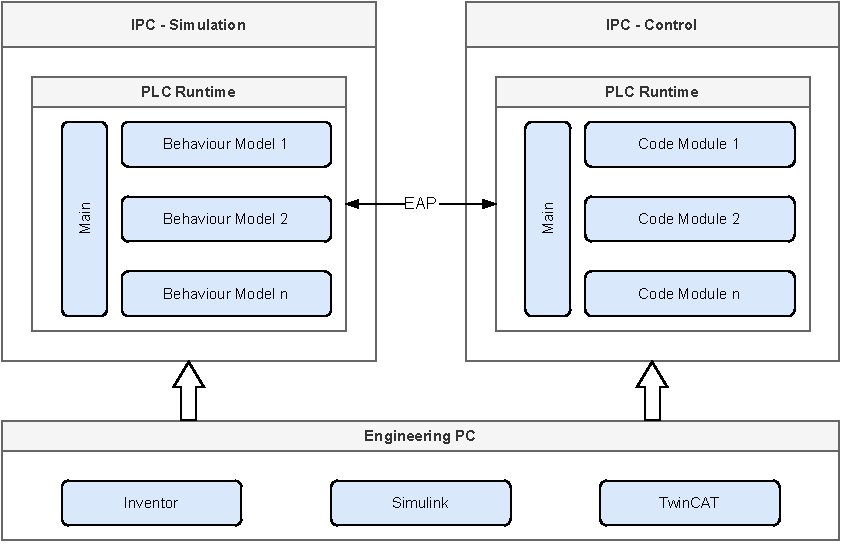
\includegraphics[width=0.9\linewidth]{figures/ExampleSetupHardware.pdf}
    		\caption[Hardware setup for this example as HIL system.]{Hardware setup for this example as HIL system. It consists of two real-time capable IPCs running the plant model and the PLC control and an engineering PC. The communication between the IPCs is done vie EAP in real-time. }
} {
        	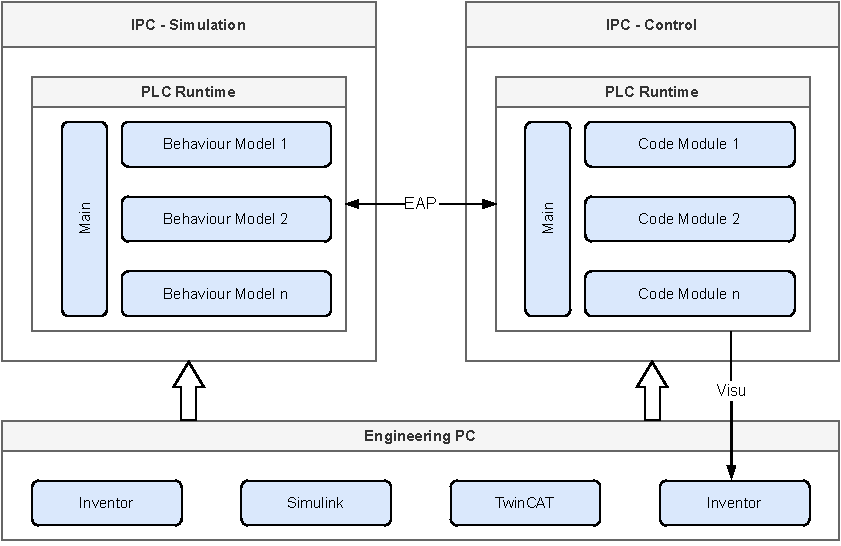
\includegraphics[width=0.9\linewidth]{figures/ExampleSetupHardwareVisu.pdf}
    		\caption[Hardware setup for this example as HIL system.]{Hardware setup for this example as HIL system. It consists of two real-time capable IPCs running the plant model and the PLC control and an engineering PC for the visualization and the development of the PLC code. The communication between the IPCs is done vie EAP in real-time. }
}
    		\label{fig:ExampleUsedSetup}
    	\end{figure}

        
%        The physical setup for the virtual commissioning consists of two real-time capable industrial PCs (IPC) on which the \textit{TwinCAT} run-time is executed. The control software to be tested is executed on the first IPC and the model of the plant is calculated on the second, thereby creating an HIL system. The communication between the two IPCs takes place in real-time via the EtherCAT Automation Protocol (EAP) \cite{TwincatEAP}. The \textit{TwinCAT} projects for both IPCs are written on an engineering PC and then loaded onto the two IPCs.


    	
    % Model
    The integration of the model description from a \textit{.fmu} file into a PLC project is done using a own product called \textit{TE1420} for a \textit{Beckhoff} PLC. With the help of this product a \textit{TcCom} object is created, which can then be integrated in TwinCAT. The inputs and outputs from this object are the same as the description from the original \textit{.fmu} file. \\
    At the time of writing this thesis, the \textit{TE1420} product is still in development and therefore cannot be used for this example. As an alternative, code generation from \textit{Simulink} and the product \textit{TE1400} is used, in order to create a \textit{TcCom} object directly from the source model in \textit{Simulink}. Thus, the generation of this \textit{TcCom} object is slightly different in the alternative, but the further use is identical. A limitation of this alternative is the mandatory use of \textit{Simulink} for the model description. The comparison between the ideal way and the alternative code generation is found in \autoref{fig:ExampleComparisonModelToPlc}.
 	\begin{figure}[htp]
		\centering
		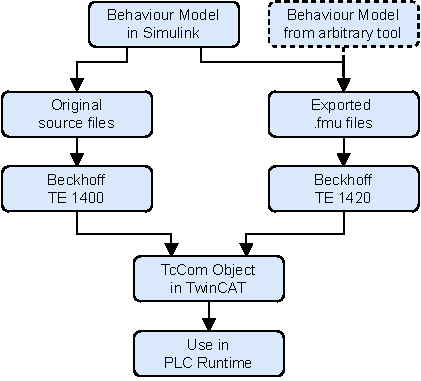
\includegraphics[width=0.5\linewidth]{figures/ComparisonIncludeFmu.pdf}
		\caption[Comparison of the integration of the physical models in \textit{TwinCAT}.]{Comparison of the integration of the physical models in \textit{TwinCAT}. Instead of using a \textit{.fmu} file to create a \textit{TcCom} object, the original source from \textit{Simulink} is used.}
		\label{fig:ExampleComparisonModelToPlc}
	\end{figure}
	
	
\section{Creation of the Data Structure - Workflow of a Manufacturer}	    \label{sec:ExampleCreateDataStructure}
    % Allgemeine Infos
    In this section the data structure for the exchange is generated. This structure consists of the CAD data, the behaviour model and source code for a PLC as described in \autoref{sec:DataStructure}. The export of the data is done from the view of a supplier or transmitter. \\
    
    % CAD
    For exporting the CAD data, this example uses the native format of \textit{Inventor} for kinematized models. That is based on the assumption that the transmitter and receiver of the data structure both use \textit{Inventor}. The structure of the assembly corresponds to the desired kinematization, taking into account required degrees of freedom. If the assembly is purely static and thus no kinematicization is required, the \textit{.step} format is used for exchange. This also simplifies the structure of the assembly, whereby logically linked components are bundled into individual assemblies. The export to the \textit{.step} format is done using the instruction \cite{InventorAnleitungExportStep} and to the native exchange format using the instruction \cite{InventorAnleitungExportPackAndGo}. \\
    
    % Verhaltensmodell
    As already mentioned, in this example the original models from \textit{Simulink} are used as an alternative for the integration into \textit{TwinCAT}. However, the behaviour model is exported as intended as a \textit{.fmu} file and included in the data structure. This is done according to the instructions \cite{MatlabFmuExport}, using a \textit{fixed-step} solver with the step size of \SI{10}{\milli\second}. The step size corresponds to the cycle time of the PLC. \\
    The interface of the models reproduces the signals of the real hardware and describes the given system. In addition, some purely virtual variables are used, which are useful for higher-level control. The level of detail can be arbitrarily precise, whereby the increasing complexity of the required calculations must be taken into account. \\
    
    % PLC 
    The source code of the PLC is exported to the \textit{PLCopen} format for exchange. Instructions for this are provided by \cite{TwincatExportPlcopen}.

    
\subsection{Module \textit{Separation}}
\subsubsection{CAD Data}
    The CAD model is built based on the desired kinematics of the pistons. In this case, the two pistons each represent a separate assembly to allow easier maintenance and use. As mentioned earlier, the assembly is exported in the native format of \textit{Inventor} based on the desired kinematics and bundled in a \textit{.zip} file. 
 %   The CAD model is built according to the desired kinematics, with the sliders of the two pistons each representing a separate sub-assemblies. The remaining components can be grouped in a separate assembly. Thus, the overall assembly \textit{Separation} consists in total of three sub-assemblies, which simplifies the kinematicization significantly. Also possible changes to the design and kinematization can be easily applied with this hierarchy of components.\\
 %   The \textit{Pack and Go} tool from \textit{Inventor} is now used to export the final CAD data. This tool gathers all relevant components of the assembly and bundles them into one folder. Additionally, this folder can be automatically compressed to a \textit{.zip} file, as is done in this case. 
    
    
\subsubsection{Behaviour Model}
% Verhaltensmodell
    The behaviour model in this case is created in \textit{Simulink} and takes into account the influence of gravity on the containers in the incoming storage. Also taken into account is the influence of the actuators on the selected position of the containers in the storage and the resulting signal from the sensors. The entire model with the inputs and outputs is shown in \autoref{fig:ModuleSeperationBehaviourModel}.  \\
    
% Interface
    %The interface of the model consists of the designated inputs and outputs of the PLC to the hardware. This ensures that the software can be tested as close as possible to reality and possible errors in the software can be corrected at an early stage. \\
    For this module, the interface consists of digital outputs for moving the two pistons and digital inputs for each of the three proximity sensors. Furthermore, additional signals are needed for the creation and deletion of the containers. These signals are purely virtual and are thus not connected to the hardware, but are required only in the logic of the module.\\
  %  The creation of the containers is equivalent to the insertion of a container into the input storage and is done in reality by the human user. If a rising edge is now detected by this signal, a container is created in the top storage location. According to the logic of the model, this container then falls down to the lower storage locations and the sensor signals are set. \\
  %  The removal of the containers corresponds to the transfer to the next module of the \textit{filling} and must be set by a higher-level controller. This means that as soon as a container is placed on the lowest position, the lower piston is opened and a rising edge is detected at this signal, this container is removed in the logic of the \textit{separation}. This signal can be used to simulate the placement of a container on the conveyor belt of the next station, whereby the conveyor belt is not in motion and thus the container is not physically removed. \\ 
    
% Beschreibung Model
  %  The model of the \textit{separation} itself consists of the logic that determines the behavior and thus the output signals of the sensors and the models of the two actuators. For modeling the actuators, the two signals for retraction and extension are processed and a virtual end switch is set accordingly. These end switches are further used in the logic of the module and do not exist in reality.  \\
	\begin{figure}[htp]
		\centering
		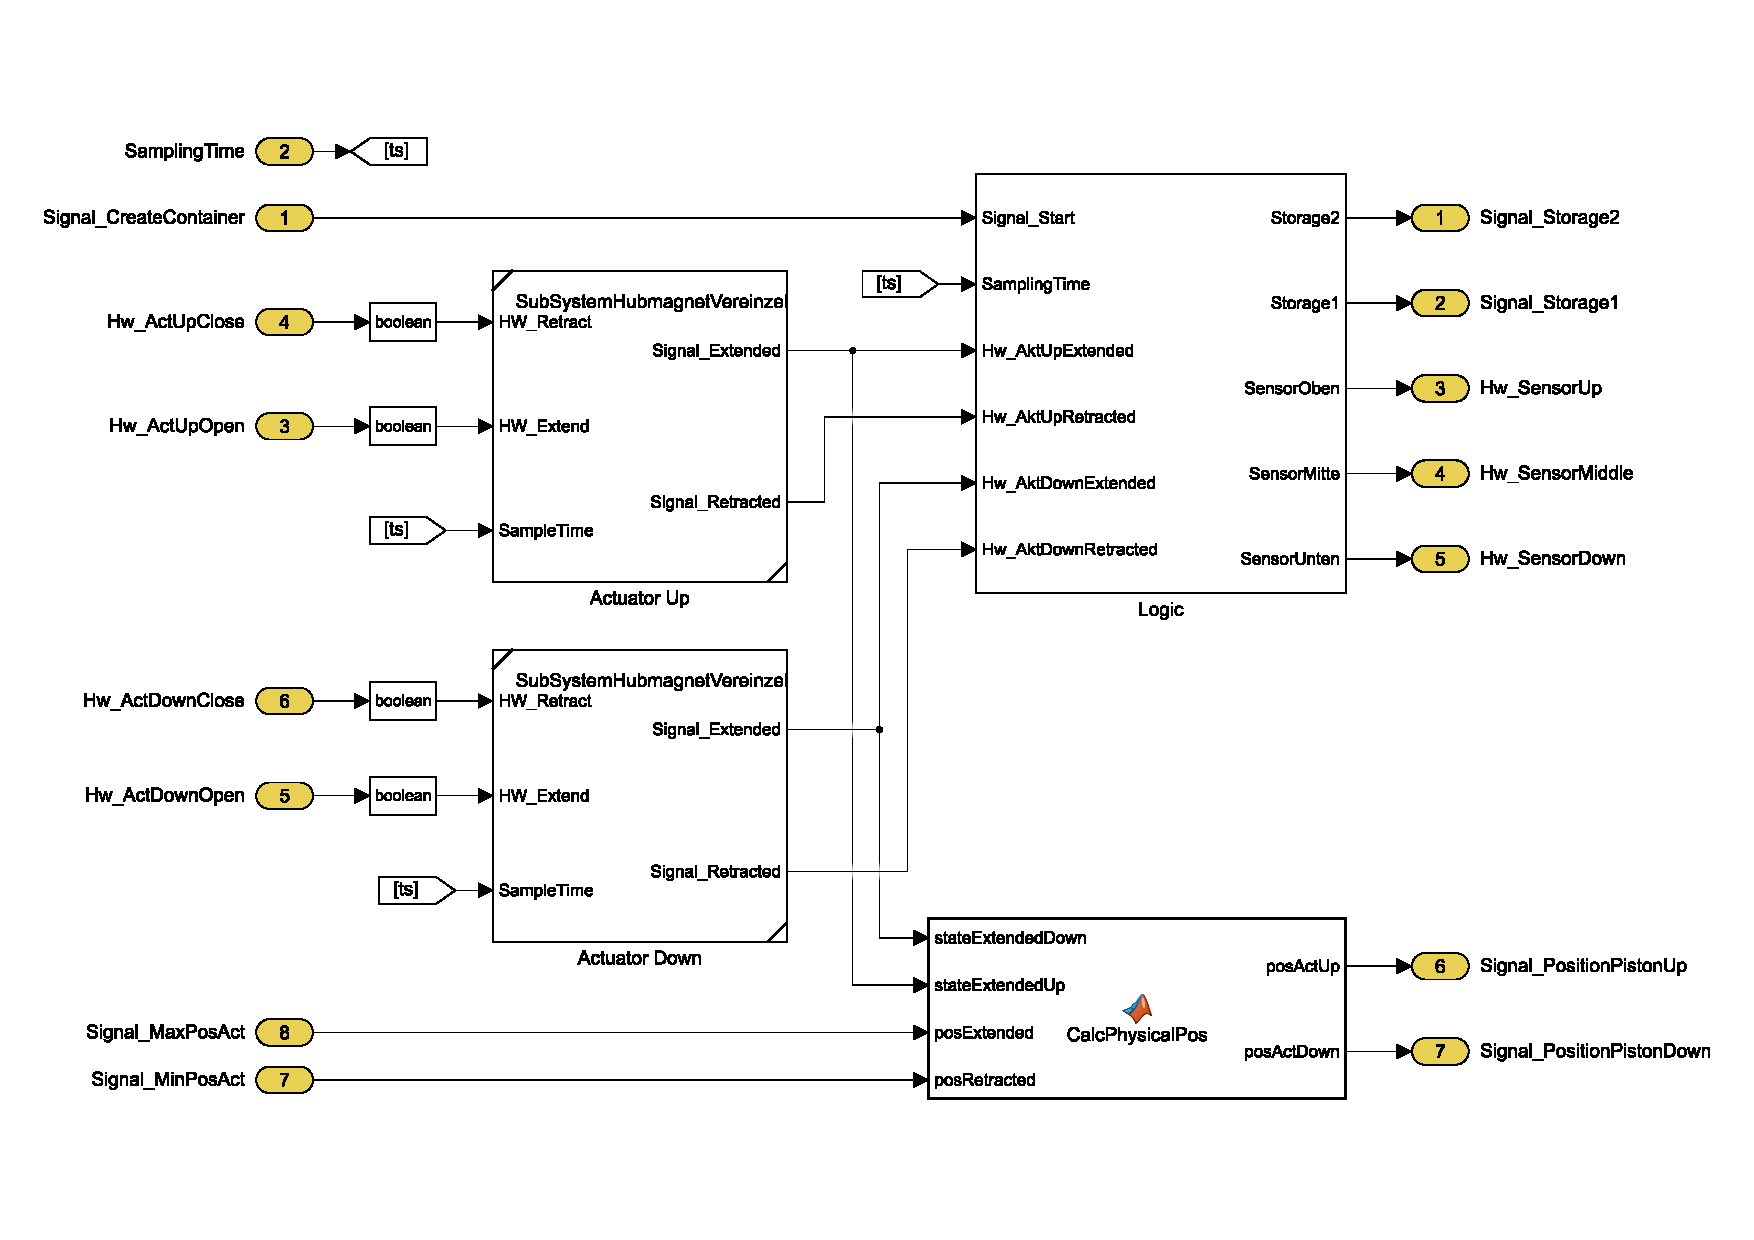
\includegraphics[trim=0mm 20mm 0mm 20mm, clip, width=0.95\linewidth]{figures/BehaviourModelSeperation.pdf}
		\caption[Behaviour model of module \textit{Separation}.]{Behaviour model of module \textit{Separation} describing the physical pistons and the logic of the input storage.}
		\label{fig:ModuleSeperationBehaviourModel}
	\end{figure}
	

% Export zu FMI
 %   As described in \autoref{sec:DataStructure}, the \textit{Simulink} model must be exported to a \textit{FMI} file, in order to create an interface that is as easily accessible as possible. This export is done according to the instructions \cite{MatlabFmuExport} and results in a \textit{.fmu} file. For a successful export of the model the solver must be set to \textit{fixed-step} and the step size must correspond to the task time of the PLC or at least be dividable by it. 
    
\subsubsection{PLC Code}
    For the exemplary control of the \textit{separation} a \textit{function block} is created. By structuring the control as a \textit{function block}, an instance of the \textit{separation} can easily be created and used in a higher-level controller. This code basically consists of a state machine in which the two pistons are controlled depending on the current state and the sensor inputs. The resulting \textit{.xml} file is listed in \autoref{lst:FbSeperation}. 

\subsubsection{Resulting File}
    The generated information of the CAD model, behaviour and control are now bundled in the proposed data structure from \autoref{sec:DataStructure}. The resulting structure for this module is shown in \autoref{fig:ExampleVereinzelungFile}. 
	\begin{figure}[htp]
		\centering
		\footnotesize
        \begin{forest}
            for tree={font=\footnotesize, grow'=0,
            folder indent=.9em, folder icons,
            edge=densely dotted}
            [ModuleSeperation.zip
                [CAD\_Data
                    [PureGeometry.step, is file]
                    [NativeInventor.zip, is file]
                ]
              [PLC\_Code
                  [FB\_Separator.xml, is file]
                  [State.xml, is file]
                  [StateSeparator.xml, is file]
               ]
              [BehaviourModel
                [ExchangeModel.fmu, is file]
                [OriginalSimulinkModel.zip, is file]
              ]
              [Documentation
              ]
            ]
          \end{forest}
		\caption[Data structure of module \textit{Separation}.] {Data structure of module \textit{Separation} consisting of CAD data as pure geometry and including kinematization in a native format, PLC code and the behaviour model as \textit{.fmu} and original \textit{Simulink} files. Additional documentation for this module is not needed resulting in an empty directory. } 
		\label{fig:ExampleVereinzelungFile}
	\end{figure}
    

\subsection{Module \textit{Conveyor Belt}}
\subsubsection{CAD Data}
    In this module the CAD model of the conveyor belt itself is provided by the manufacturer and integrated in the assembly. The three sliders of the stoppers form again a sub-assembly to simplify the kinematization. The conveyor itself does not need any additional kinematization. The remaining components such as the conveyor itself, the attachment, and the sensors are bundled into a second assembly to avoid any obstacles to the kinematics. The three \textit{dosing units} are also represented as a own sub-assembly. \\
  
   Since the kinematics of the pistons are supposed to be exported in this example as well, the native CAD format is kept. Alternatively, a pure exchange of the geometry with an \textit{.step} file can be done.
   % In contrast to the previous example, in this station the CAD design is exported without kinematics since the supplier only provides the pure 3D geometry. This is the case, for example, when the customer and the supplier use different CAD tools and thus the native file formats are not compatible. In this situation, the customer has to create the kinematization according to his needs. For the export without the kinematization, the \textit{.step} format is selected due to its wide compatibility and the process is done according to the instruction \cite{InventorAnleitungExportStep}. 
    
\subsubsection{Behaviour Model}
    The behaviour model in this module consists of the DC motor of the conveyor belt, a generic drive for the dosing units and a logical combination of the pistons and sensors. The final model in \textit{Simulink} is shown in \autoref{fig:ExampleFillingModelDrive}. The modeling of the DC motor is similar to this example from the Matlab documentation \cite{SimulinkExampleDcMotorControl}, using the characteristics from the data sheet of the used motor \cite{DataSheetDCMotor}. \\
    The stepper motors of the dosing units are not modeled as detailed as the DC motor and therefore use a generic description, which also results in a reduction of the required computing power. \\
    
    %The interface for the DC motor consists of the input voltage expressed in the unit \si{\volt} and the velocity on the conveyor belt in \si{\milli\meter\per\second}. Since the angular velocity of the motor axis in \si{\radian\per\second} is used in the model of the motor, a transformation of the units into a linear velocity on the conveyor belt is performed. This transformation represents the gear of the conveyor belt and consists of a constant coefficient in \textit{Simulink}. \\

   % The model of the DC motor consists of three parts in a feedback loop: a transfer function of the armature, a transfer function of the load and the feedback to the input voltage as a result of the back electromotive force (back EMF). This approach to modeling is kept simple, but represents the behaviour of the motor with sufficient accuracy for this purpose. However, if needed, the modeling can be further deepened and improved without problems. \\
  %  The transfer function of the armature $G(s)$ transforms the input voltage $V_{in}$ by means of the torque constant $k_m = \SI{56.1}{\milli\newton\meter\per\ampere}$, the inductance of the windings $L = \SI{1.05}{\henry}$ and the electrical resistance $R = \SI{31.2}{\ohm}$ into a torque $\tau$. This torque further acts as an input to the transfer function of the load $H(s)$ with the resulting angular velocity $\omega$ of the motor axis. The movement of the motor axis itself generates a back EMF reducing the input voltage at the armature. This voltage is determined by the back-EMF constant $K_b = \SI{5.87}{\milli\volt\per\minute}$ and the velocity of the motor axis, and is subtracted from the input voltage of the armature. \\
  %  Using the characteristic values from the data sheet of the motor, the following transfer function of the armature $G(s)_{Armature}$ is derived and the transfer function of the load $H(s)_{Load}$ is determined based on the real behavior of the motor with:
 %   \begin{align}
 %       G(s)_{Armature} &= \frac{k_m}{L s + R} = \frac{56.1\cdot 10^{-3}}{1.05 s + 31.2} \\
 %       H(s)_{Load} &= \frac{1}{J s + k_f} = \frac{1}{0.02 s + 0.2}
 %   \end{align}
    
 %   With these two transfer functions and the information from the data sheet, the model of the motor is created.
	\begin{figure}[htp]
		\centering
		\begin{subfigure}{.95\textwidth}
			\centering
            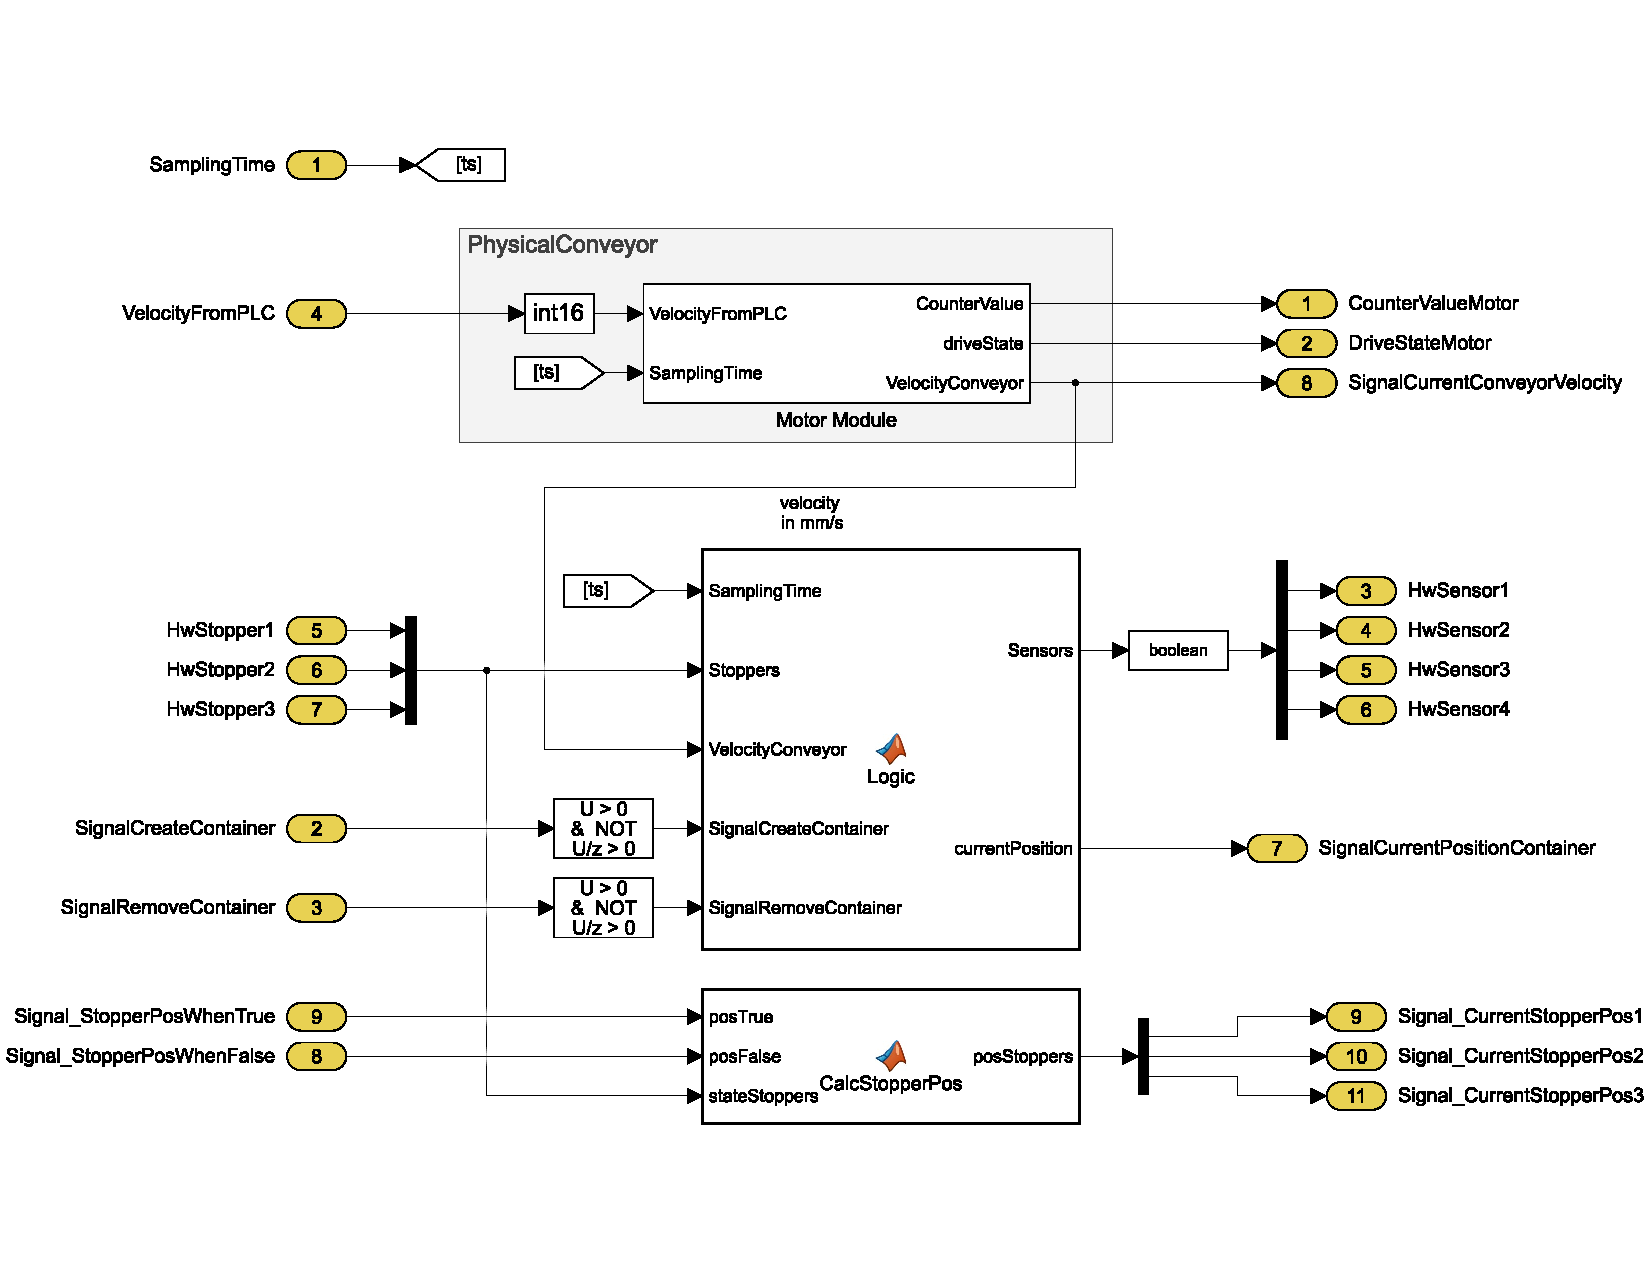
\includegraphics[trim=0mm 20mm 0mm 20mm, clip, width=0.95\linewidth]{figures/BehaviourModelConveyor.pdf}
			\caption{Conveyor Belt}
		\end{subfigure}
		\vspace{3mm}
		
		\begin{subfigure}{.85\textwidth}
			\centering
            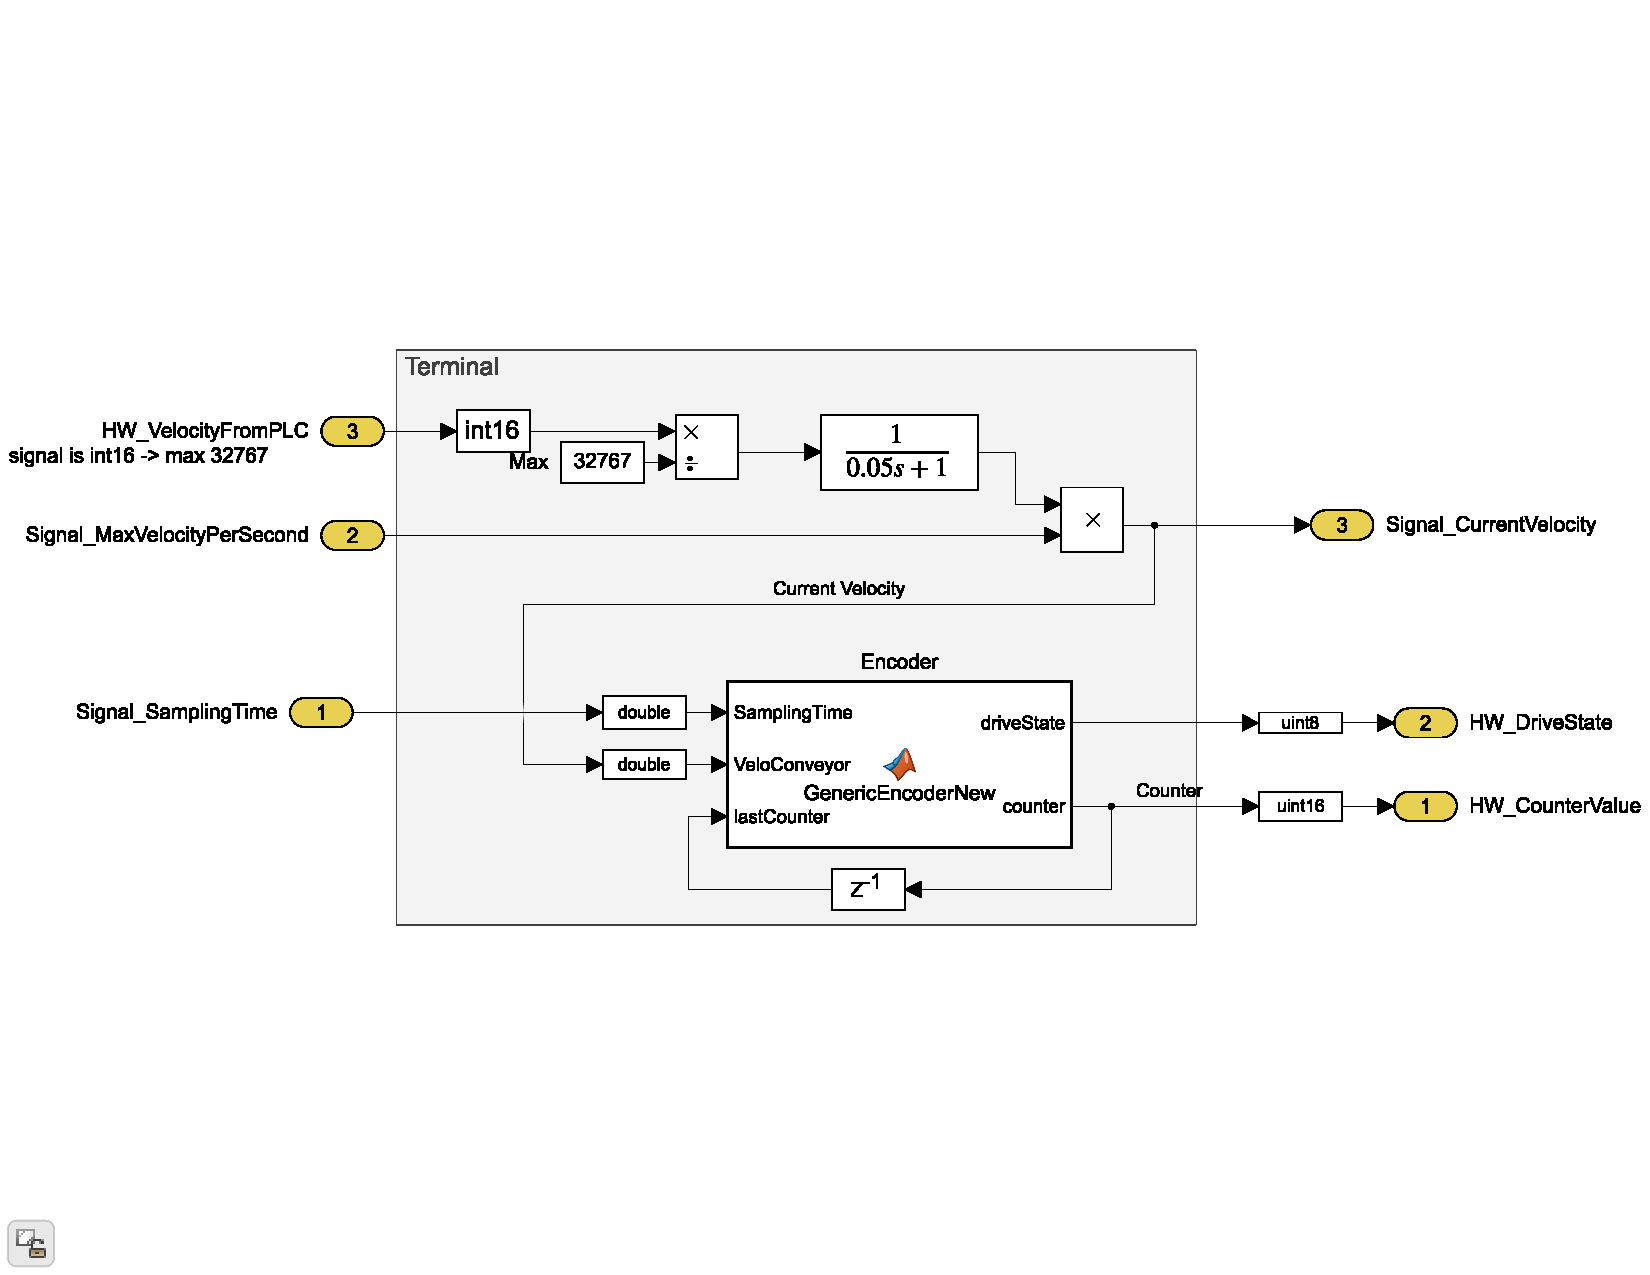
\includegraphics[trim=0mm 55mm 0mm 55mm, clip, width=0.95\linewidth]{figures/BehaviourModelDosingUnit.pdf}
			\caption{Dosing Unit}
		\end{subfigure}
		\caption[Behaviour model of module \textit{Conveyor Belt}.] {Behaviour model of module \textit{Conveyor Belt} describing the DC motor of the conveyor belt and the stepper motor of the \textit{dosing units}. }
		\label{fig:ExampleFillingModelDrive}
	\end{figure}
	
%	As already shown in the previous example and described in \autoref{sec:DataStructure} the model must be exported from \textit{Simulink}. The export is again done according to the instruction \cite{MatlabFmuExport} and results in a \textit{.fmu} file. Again, the solver must be set to type \textit{fixed-step} and the step size must be dividable by the used task time of the PLC. In this case the step size is equal to the task time with \SI{10}{\milli\second}. 
    
    
\subsubsection{PLC Code}
   The PLC code in this module consists of two \textit{function blocks}: one block for the \textit{conveyor belt} and one block for the \textit{dosing units}. The functionality of these blocks consists in the initialization of the motors and the movement with a constant speed for the conveyor belt and the traveling of a defined distance for the dosing units. The linking of these blocks remains the customer's task and is not supplied by the manufacturer. The two \textit{function blocks} are listed in \textit{PLCopen} format in \autoref{lst:FbConveyorBelt} and \autoref{lst:FbSDosingUnit}. 
  
 %  In this module the manufacturer only offers the hardware with the behaviour model, but no PLC code. Therefore, the development of the control code is the task of the customer and this part of the data exchange remains empty. \\
  % This scenario can also occur in practice if the supplier only produces the hardware and the creation of PLC code is not part of his product portfolio, or he does not support the \textit{PLCopen} format. In this case it results in additional work for the customer, but does not cause any additional problems. 
  
\subsubsection{Resulting File}
  The collected information is now merged into the proposed data structure. This data structure is shown in \autoref{fig:ExampleFillingFile} and consists of the CAD assembly, the behaviour model and PLC code. In addition some documentation is attached to the data structure.
	\begin{figure}[htp]
		\centering
		%\footnotesize
        \begin{forest}
            for tree={font=\footnotesize, grow'=0,
            folder indent=.9em, folder icons,
            edge=densely dotted}
            [ModuleConveyorBelt.zip
                [CAD\_Data
                    [PureGeometry.step, is file]
                    [NativeInventor.zip, is file]
                ]
                [PLC\_Code
                    [FB\_Conveyor.xml, is file]
                    [FB\_Dispenser.xml, is file]
                    [State.xml, is file]
                    [StateCnv.xml, is file]
                    [StateDisp.xml, is file]
                ]
                [BehaviourModel
                    [ExchangeModel.fmu, is file]
                    [OriginalSimulinkModel.zip, is file]
                ]
              [Documentation
                  [Datasheet\_DCMotor.pdf, is file]
                  [Datasheet\_EncoderMotor.pdf, is file]
                  [Datasheet\_DosingStepperMotor.pdf, is file]
              ]
            ]
          \end{forest}
		\caption[Data structure of module \textit{Conveyor Belt}.] {Data structure of module \textit{Conveyor Belt}consisting of CAD data as pure geometry and including kinematization in a native format, PLC code, the behaviour model exported to a \textit{.fmu} file and the original source from \textit{Simulink} and additional documentation.}
		\label{fig:ExampleFillingFile}
	\end{figure}
	

\subsection{Module \textit{Cartesian Gripper}}
    \subsubsection{CAD Data}
    Similar to the previous modules, the structure of the CAD data reflects the desired kinematization. For this reason, the \textit{cartesian gripper} consists of three assemblies for the respective axes and one for the remaining components. The degrees of freedom of the three axes are restricted to the desired direction of motion. Since the CAD data along with the kinematization will be sent to the customer, the native \textit{Inventor} format is used again.
    
    \subsubsection{Behaviour Model}
    The behaviour model of the \textit{cartesian gripper} describe the three axes of motion and the gripper itself. In the process, a stepper motor is merged with the terminal of the PLC into one model and described generically. As a result of the generic model, the level of detail is reduced and so is the complexity of the calculation. Furthermore, the generic model is independent of the selected motor type.
    	\begin{figure}[htp]
		\centering
		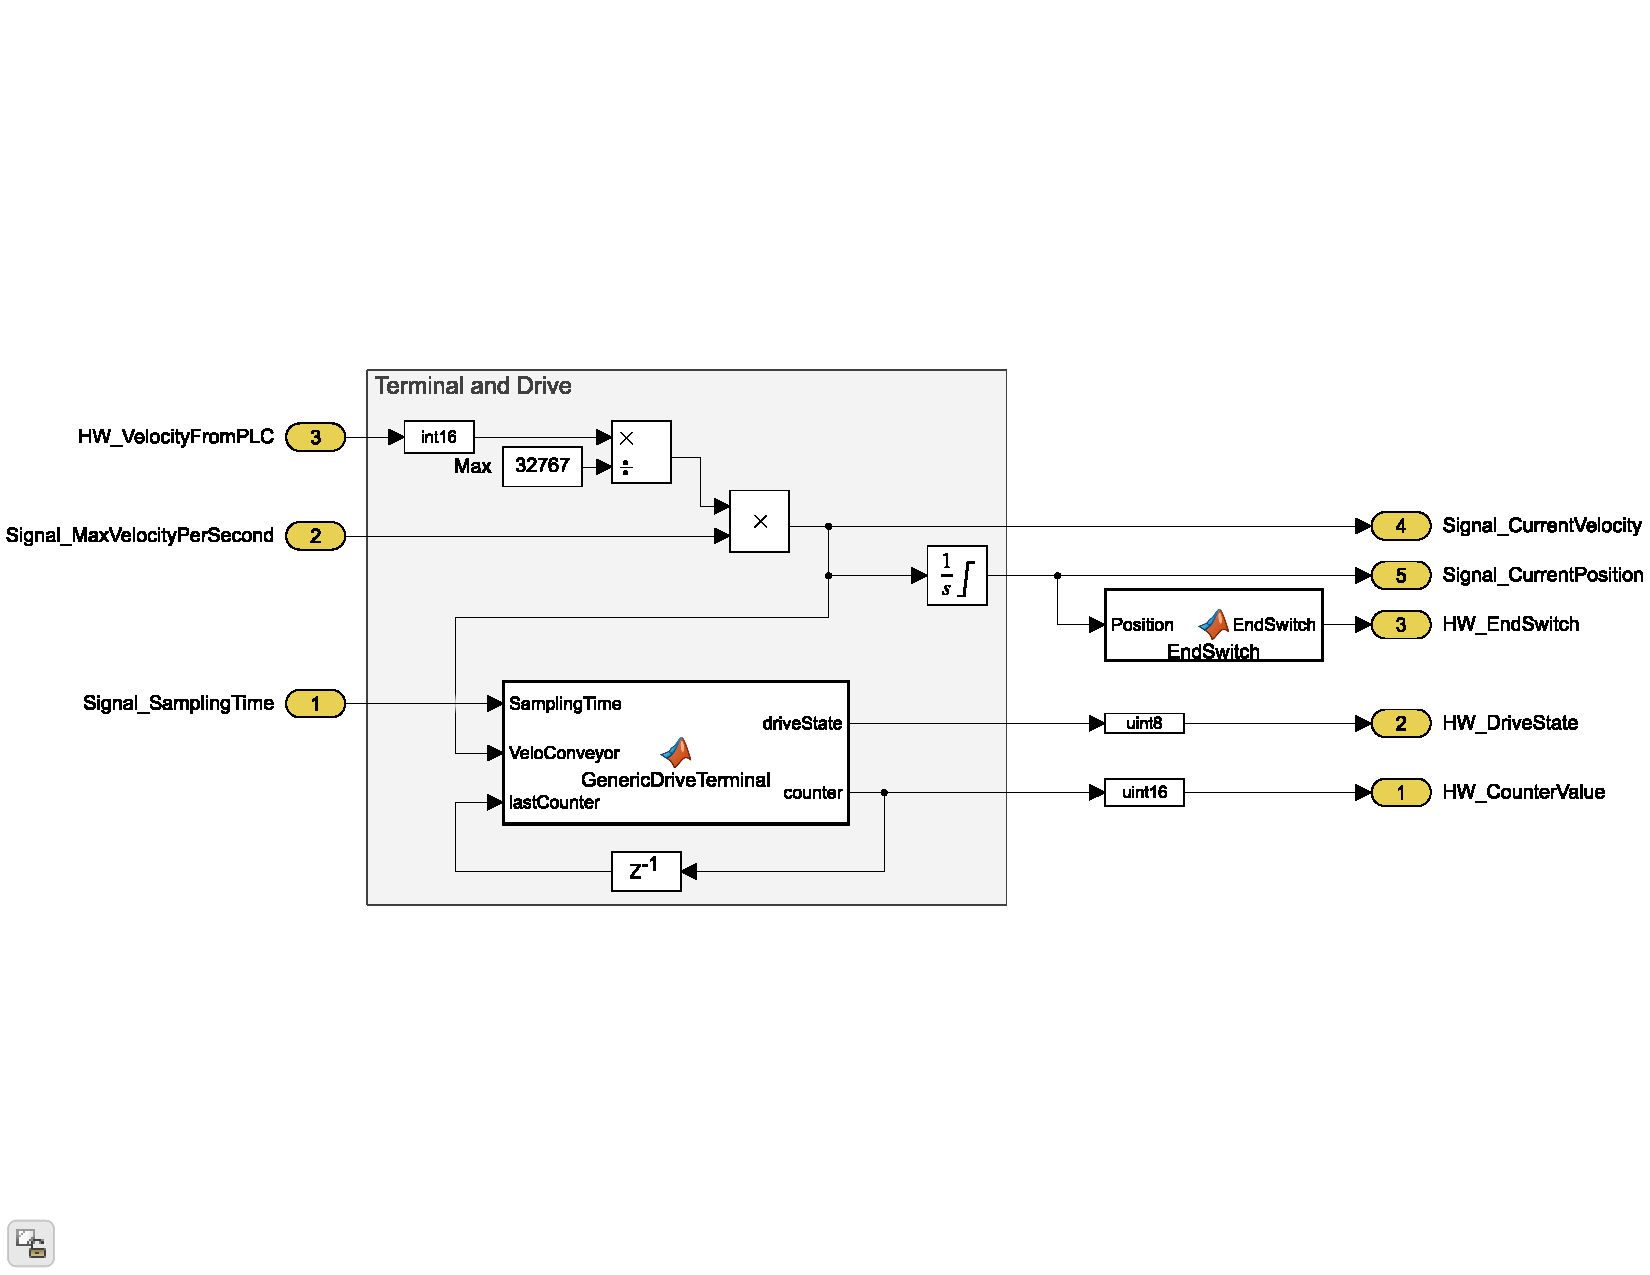
\includegraphics[trim= 0mm 60mm 0mm 60mm, clip, width=0.95\linewidth]{figures/BehaviourModelKinGripper.pdf}
		\caption[Behaviour model for module \textit{Cartesian Gripper}.] {Behaviour model for module \textit{Cartesian Gripper} describing a generic motor merged with a PLC motor terminal.}
		\label{fig:ModuleCarthesianGripperBehaviourModel}
	\end{figure}
	
	%	Wie auch schon zuvor wird schließlich das Modell in eine \textit{.fmu} Datei exportiert laut \autoref{sec:DataStructure} und \cite{MatlabFmuExport}. Im Unterschied zu den vorangeganenen Modulen wird hier eine schnellere step size mit  \SI{2}{\milli\second} für den \textit{fixed-step} solver gewählt. 
	
	\subsubsection{PLC Code}
	In this module, a \textit{function block} is provided for controlling a motor axis, where this block controls only one axis and must be instantiated later for each motor. This block thereby independently performs the homing to a reference zero allowing an accurate movement to a target point with a desired speed. Again, the control is exported to the \textit{PLCopen} format and is listed in \autoref{lst:FbManipulatorAxis}.
	
	\subsubsection{Resulting File}
	The last step is now to merge the data into the proposed data structure from \autoref{sec:DataStructure}. This structure is shown in \autoref{fig:ExampleCarthesianGripperFile} and consists again of the CAD assembly, the behaviour model and source code for a PLC.
	\begin{figure}[htp]
		\centering
		\footnotesize
        \begin{forest}
            for tree={font=\footnotesize, grow'=0,
            folder indent=.9em, folder icons,
            edge=densely dotted}
            [ModuleCartesianGripper.zip
                [CAD\_Data
                    [PureGeometry.step, is file]
                    [NativeInventor.zip, is file]
                ]
              [PLC\_Code
                  [FB\_ManipulatorAxis.xml, is file]
                  [State.xml, is file]
                  [StateMan.xml, is file]
               ]
              [BehaviourModel
                [ExchangeModel.fmu, is file]
                [OriginalSimulinkModel.zip, is file]
              ]
              [Documentation
              ]
            ]
          \end{forest}
		\caption[Data structure of module \textit{Cartesian Gripper}.] {Data structure of module \textit{Cartesian Gripper} consisting of the pure geometry and included kinematization in a native format, PLC code and the behaviour model exported to a \textit{.fmu} file and the original source files from \textit{Simulink}. The folder of additional documentation is also empty in this module.}
		\label{fig:ExampleCarthesianGripperFile}
	\end{figure}


  
    
    
\subsection{Module \textit{Load Cell}}
    \subsubsection{CAD Data}
    Since no kinematization is required for this module, no special steps are necessary in the construction of the CAD assembly. In addition, data exchange is simplified since a \textit{.step} file can be used without losing any relevant information.
    
    \subsubsection{Behaviour Model}
    The generation of the behaviour model of this module is similarly simple, because the serial communication itself is not modeled but only the message as \textit{string}-type for debugging purpose. With this behaviour model shown in \autoref{fig:ModuleLoadCellBehaviourModel} a message can be created with a defined prefix and suffix and a desired measured value, which later has to be interpreted by the PLC.
	\begin{figure}[htp]
		\centering
		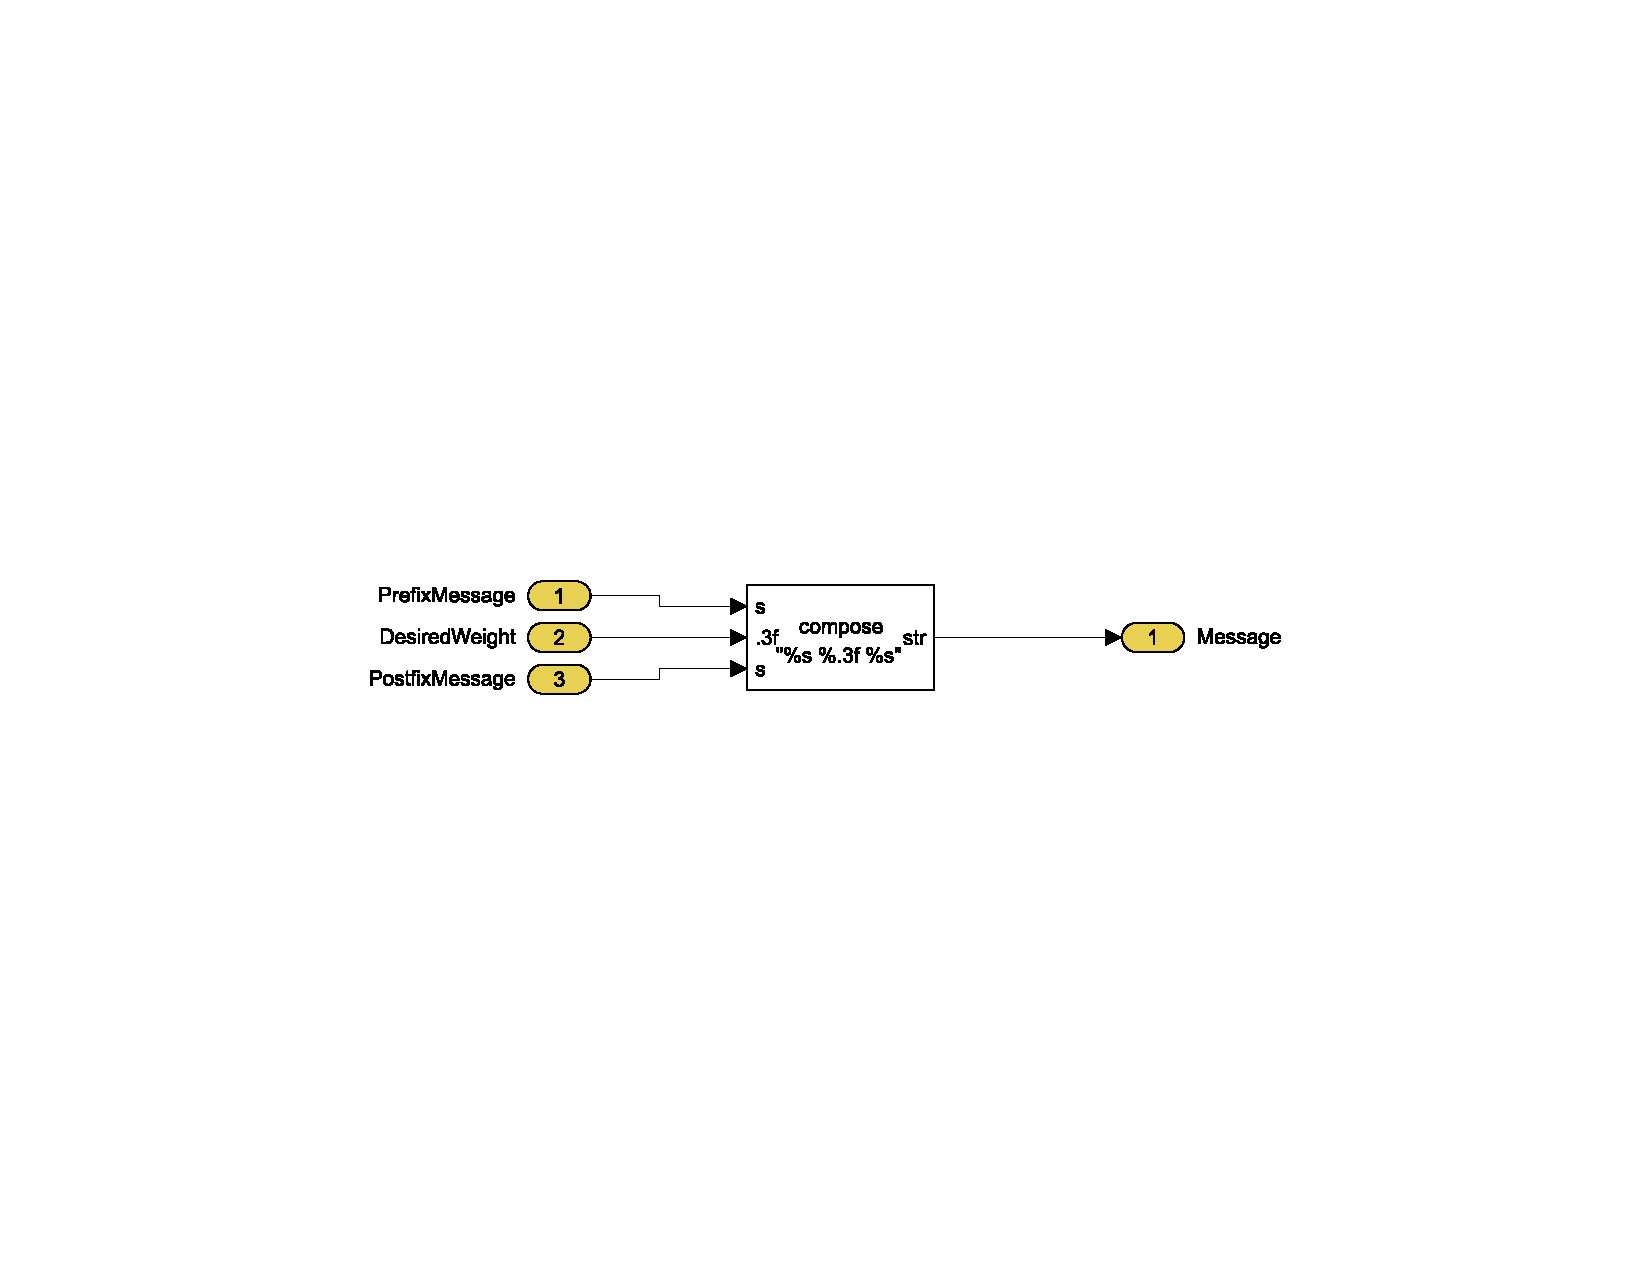
\includegraphics[trim=60mm 95mm 60mm 95mm, clip, width=0.65\linewidth]{figures/BehaviourModelLoadCell.pdf}
		\caption[Behaviour model of module \textit{Load Cell}.]{Behaviour model of module \textit{Load Cell} consisting of composing a serial message with the measured weight.}
		\label{fig:ModuleLoadCellBehaviourModel}
	\end{figure}
	
	\subsubsection{PLC Code}
	Here the manufacturer provides only the hardware and the documentation of the communication, but no code for the PLC. 
	
	\subsubsection{Resulting File}
    Also in this module the last step consists of merging the data into the data structure. The resulting structure is shown in \autoref{fig:ExampleLoadCellFile} and consists of the CAD assembly, the behaviour model and additional documentation. 
	\begin{figure}[htp]
		\centering
		\footnotesize
        \begin{forest}
            for tree={font=\footnotesize, grow'=0,
            folder indent=.9em, folder icons,
            edge=densely dotted}
            [ModuleLoadCell.zip
                [CAD\_Data
                  [PureGeometry.step, is file]
                ]
                [BehaviourModel
                  [ExchangeModel.fmu, is file]
                   [OriginalSimulinkModel.zip, is file]
                ]
                [Documentation
                    [SerialCommunication.pdf, is file]
                ]
            ]
          \end{forest}
		\caption[Data structure of module \textit{Load Cell}.] {Data structure of module \textit{Load Cell} consisting of the pure geometry, the behaviour model as exported \textit{.fmu} file and the original source in \textit{Simulink} and some documentation. }
		\label{fig:ExampleLoadCellFile}
	\end{figure}
	
	

	
    
\subsection{Module \textit{Thermal Processing}}
    \subsubsection{CAD Data}
    This module is also based on static components and therefore has no kinematization. This simplifies on the one hand the setup in the CAD software and on the other hand the export of the assembly. As a result, no special requirements for the CAD model are needed and the export can be performed in the \textit{.step} format without the loss of relevant information.
    
    \subsubsection{Behaviour Model}
    However, the behaviour model is slightly more complex with the modeling of the temperature curve. Taking into account the room temperature and the maximum reachable temperature of the cartridge heaters, the temperature of the containers is described with a transfer function. Finally, this temperature has to be converted into the corresponding signals of the sensors. The entire model in \textit{Simulink} is shown in \autoref{fig:ModuleThermalProcessingBehaviourModel}.
	\begin{figure}[htp]
		\centering
		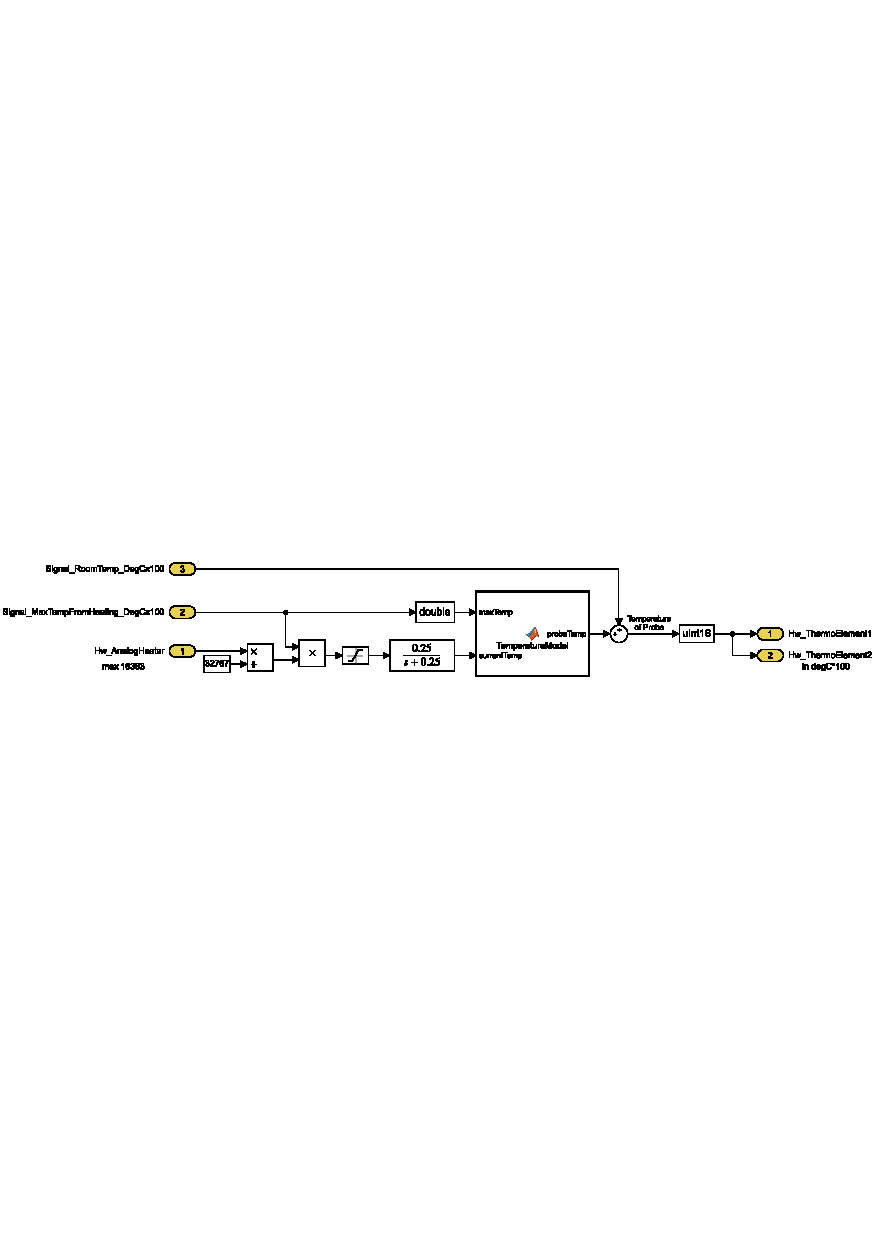
\includegraphics[trim=0mm 93mm 0mm 93mm, clip, width=0.95\linewidth]{figures/BehaviourModelThermalProcessing.pdf}
		\caption[Behaviour model of module \textit{Thermal Processing}.] {Behaviour model of module \textit{Thermal Processing} describing the temperature curve of a container with the influence of the used heating cartridges and the resulting sensor signals.}
		\label{fig:ModuleThermalProcessingBehaviourModel}
	\end{figure}
	
    
    \subsubsection{PLC Code}
    With this module the PLC code is again provided in the form of a \textit{function block}. This block is listed in \autoref{lst:FbManipulatorAxis} and enables the initialization and operation of the module. In the process, the containers are heated to a defined temperature and then held for a certain time. 
    
    
    \subsubsection{Resulting File}
    Finally, the collected data is merged into the data structure. This structure is shown in \autoref{fig:ExampleThermalProcessingFile} and consists of CAD data, behaviour model and PLC code.
	\begin{figure}[htp]
		\centering
		\footnotesize
        \begin{forest}
            for tree={font=\footnotesize, grow'=0,
            folder indent=.9em, folder icons,
            edge=densely dotted}
            [ModuleThermalProcessing.zip
                [CAD\_Data
                    [PureGeometry.step, is file]
                ]
                [PLC\_Code
                 [FB\_HeatingSystem.xml, is file]
                 [State.xml, is file]
                 [StateHeat.xml, is file]
                ]
                [BehaviourModel
                    [ExchangeModel.fmu, is file]
                    [OriginalSimulinkModel.zip, is file]
                ]
                [Documentation
                ]
            ]
          \end{forest}
		\caption[Data structure of module \textit{Thermal Processing}.] {Data structure of module \textit{Thermal Processing} consisting of pure geometry, PLC code and the behaviour model as exported \textit{.fmu} file and the original source from \textit{Simulink}. Also in this module no further documentation is needed.}
		\label{fig:ExampleThermalProcessingFile}
	\end{figure}
	
	

            

\section{Implementation of the Data Structure - Workflow of a Customer}
    In this section, the data structures shown in \autoref{sec:ExampleCreateDataStructure} are now send to the receiver and used in a virtual commissioning. This is done from the perspective of a customer or receiver. \\
    
    \subsection{A Single Module}
    
    % CAD
    For the CAD data, as already mentioned, it is assumed that both sides use \textit{Inventor}. This way the native format can be kept and in addition to the geometry also the kinematization is preserved. For purely static modules without kinematization, the \textit{.step} format is used. The import of a \textit{.step} file is done using the instructions \cite{InventorAnleitungImportStep}. \\
    
    % Verhaltensmodell
    Since in this example the customer uses a PLC from manufacturer \textit{Beckhoff}, the behaviour model is integrated directly from the \textit{Simulink} files into the PLC run-time. As said, the integration of \textit{.fmu} files is not possible at this time due to ongoing development of the required product. The integration of the \textit{Simulink} models into \textit{TwinCAT} is done analog to this instruction \cite{TwincatGenerateTccom}. \\
    
    % PLC Code
    The \textit{function blocks} of the PLC control can be easily integrated and instantiated in an existing \textit{TwinCAT} project. After assigning the interface variables, the code can be used. 


%\subsection{Module \textit{Separation}}
%\subsubsection{CAD Data}
%    In this example, the receiver is also using the CAD software \textit{Inventor} and therefore the %use of native file formats is possible. Since the CAD data was generated via the \textit{Pack %and Go} tool, it can easily be imported by the customer. To do this, only the \textit{.zip} %folder containing the CAD data needs to be extracted and can then be used immediately to design %the remaining plant. By keeping the native formats, the kinematization of the assembly is %preserved and as a result, there is no need to recreate the kinematization, due to the possible %loss of data when using an unsupported data format.
%
%\subsubsection{Behaviour Model}
%    The implementation of the behavior of the station \textit{Separation} for a virtual %commissioning is done in \textit{Simulink}, as described before. The \textit{FMI} object is %integrated in \textit{Simulink} and communicates with the PLC runtime via the \textit{ADS} %interface. The model is executed separately from the PLC on an engineering system. \\
%    
%    % Modell und Einstellungen beschreiben
%    The final setup in \textit{Simulink} for virtual commissioning is shown in %\autoref{fig:ExampleSeperationUseSimulink}. It consists of the \textit{FMI} object with the %implementation of the behavior in the middle and the \textit{ADS} communication block in the %upper left. In addition, two functions are used to compress the digital signals. For this %purpose, the boolean signals to the actuators are combined in one byte by setting corresponding %bits. In the same way, the three signals from the sensors are also combined in a second byte, %with one bit representing each sensor signal. With this compression, the number of variables for %communication and thus the required time can be minimized. A further side effect of this is the %possibility of bypassing the limitation of the test license with respect to the maximum number %of variables for communication.\\
%    
%    The solver must also be set to type \textit{fixed-step} with the same step size as the task time %of the PLC, which in this case is \SI{10}{\milli\second}. \\
%    In the \textit{ADS} block the variables for communication are set according to their data %direction. For this purpose the sensor signals are written to the PLC via the command %\textit{ADS-Write} and the signals of the actuators are read from the PLC via \textit{ADS-Read}. %
%	\begin{figure}[htp]
%		\centering
%		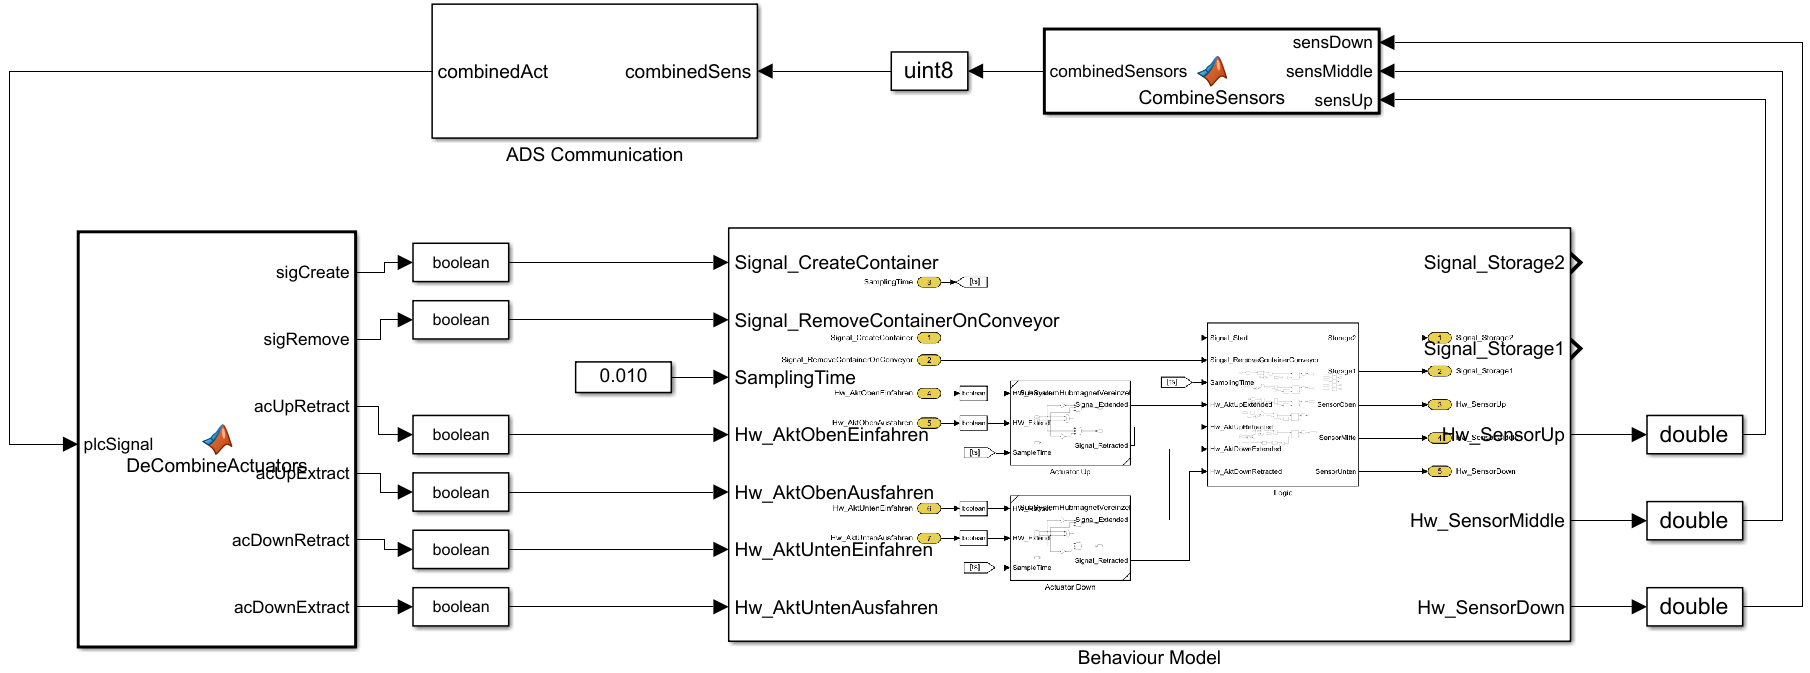
\includegraphics[width=0.95\linewidth]{figures/ExampleVereinzelungUseSimulink.PNG}
%		\caption{Use of the behaviour model in \textit{Simulink} for example \textit{Seperation}}
%		\label{fig:ExampleSeperationUseSimulink}
%	\end{figure}
%    
%    
%\subsubsection{PLC Code}
%    The integration of the exemplary control of the separation in \textit{TwinCAT} takes place in a %higher-level program, which is listed in \autoref{lst:VereinzelungSolution}. As part of this %control, the input and output variables are defined and linked to the instance of the separation %function block. Then this instance must be called periodically to determine the current state. %Besides this call, the compression of the input and output variables is also part of this %higher-level control. As already described, the signals of the sensors and actuators are each %compressed to one byte. \\
%    Finally, the virtual commissioning of the station can now be performedby testing the software.
%    \lstinputlisting[basicstyle=\tiny, caption={Main programm with included example code of example %\textit{Seperation}}, label=lst:VereinzelungSolution]{sourcecode/ExampleVereinzelungMain.xml}
%
%
%\subsection{Module \textit{Conveyor Belt}}
%\subsubsection{CAD Data}
%    The CAD data in this example is only available as a non-kinematic \textit{.step} file and as a %consequence, the customer has to create the kinematics according to his own needs. The first %step is to import the geometry of the station as a \textit{.step} file into \textit{Inventor}. %The import with the following conversion into native file formats is done according to the %instruction \cite{InventorAnleitungImportStep} and results in a native assembly in the %\textit{.iam} format with the individual parts as \textit{.ipt} files. \\
%    After importing the geometry, the assembly must be kinematized again. For this purpose, the %slide of each of the three stoppers is again combined in a separate sub-assembly. The remaining %individual parts do not require any modifications, but can also be grouped into their own %sub-assembly for simpler handling. The kinematics itself consists of the dependencies of the %stoppers, where the slides are placed concentric to the stoppers and the position of the slides %is given by a \textit{user-param}. These parameters and with them the position will be written %by the PLC later during the virtual commissioning. 
%    
%    
%\subsubsection{Behaviour Model}
%    Similarly to the previous example, the behaviour model for the virtual commissioning is created %in \textit{Simulink} on an engineering system and communicates with the PLC runtime via the %\textit{ADS} interface. The complete setup of the simulation in \textit{Simulink} for the %virtual commissioning is shown in \autoref{fig:ExampleFillingUseModel}.\\
%    
%    In the simulation for the virtual commissioning, the \textit{.fmu} file with the behaviour model %of the motor is embedded. In addition to the motor, the used PLC motor terminal has to be %modeled, because it generates the actual signals to the motor and interprets the signals of the %encoder. This model is shown in \autoref{fig:ExampleFillingKlemmeModel} and consists of the %conversion of the reference velocity into a voltage signal in the range from \SI{0}{\volt} to %\SI{48}{\volt}. Since in the real system the supply voltage of the motor is available only up to %\SI{24}{\volt}, the maximum output voltage in the model is also limited to \SI{24}{\volt}. In %the lower section, the position of the motor axis is determined by the integral of the actual %velocity of the motor over time. From this calculated position a counter variable is determined. %This integral calculus represents the real encoder on the motor axis in the model. \\
%    The motor control itself is done via an NC axis in \textit{TwinCAT}. The basic principle in the %use of an NC axis can be summarized as follows: Based on the configuration of the motor, the NC %axis generates a profile for the acceleration and, derived from this, the velocity. With this %profile, a current reference velocity is determined for each time step and sent to the PLC motor %terminal. The motor terminal transforms the reference velocity into a physical signal to the %motor. In this case, the velocity is transformed into a voltage between \SI{-24}{\volt} and %\SI{+24}{\volt}. The encoder on the motor axis is again connected to the motor terminal and %supplies a signal depending on the actual velocity. This signal is interpreted in the motor %terminal and converted into the actual position of the axis. This value of the actual position %is then returned to the NC axis and is taken into account in the calculation of the next %reference value of the velocity. \cite{TwincatNcAchsenGeneral}\\
%    
%% ADS Blöcke und Encodierung
%    The communication with the PLC is again done via the \textit{ADS} block in the upper left area. %Also in this case the necessary signals of the communication are compressed in two variables. %This means that only one variable has to be read or written per cycle, which subsequently %results in a time saving. The compression and decompression of the variables for the %communication is done in two Matlab functions by means of different bit operations. These %operations require attention to the correct data type of the different variables, which can be %seen in the various \textit{cast} blocks in the simulation. A side effect of the compression is %again the minimization of the number of variables and the thereby allowed use of the freely %available test license of \textit{TwinCAT}. \\
%    
%% Solver Settings
%    The settings of the solver for this simulation consists of setting the type \textit{fixed-step}, %where the step size again corresponds to the task time of the PLC with \SI{10}{\milli\second}. %In the \textit{ADS} block, the two variables are configured based on their direction, where the %variable \textit{PLCtoModel} is written by the PLC and thus read by the simulation with %\textit{ADS-Read} and the variable \textit{modelToPLC} should be written by the simulation and %read by the PLC with \textit{ADS-Write}. 
%	\begin{figure}[htp]
%		\centering
%		\begin{subfigure}{.95\textwidth}
%			\centering
%			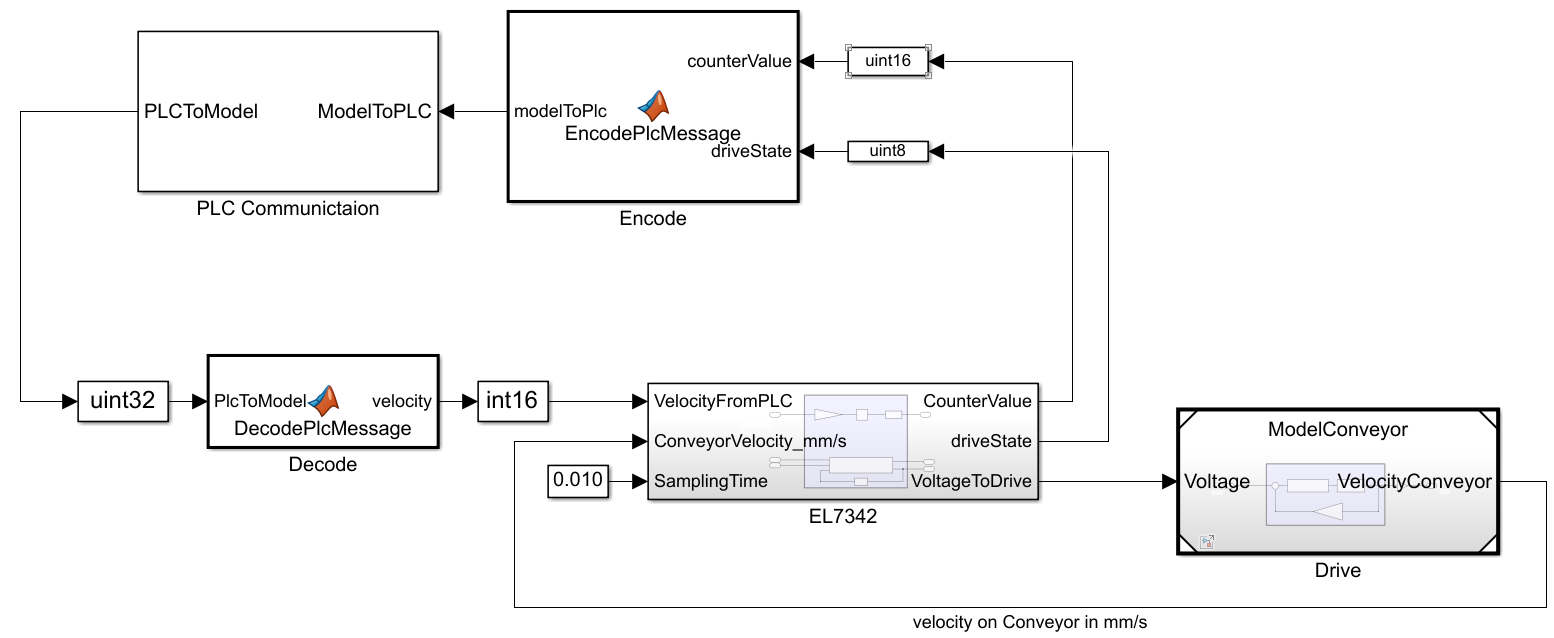
\includegraphics[width=.95\linewidth]{figures/ExampleConveyorModelComplete.PNG}
%			\caption{Complete setup}
%		\end{subfigure}
%		\vspace{3mm}
%		
%		\begin{subfigure}{.8\textwidth}
%			\centering
%			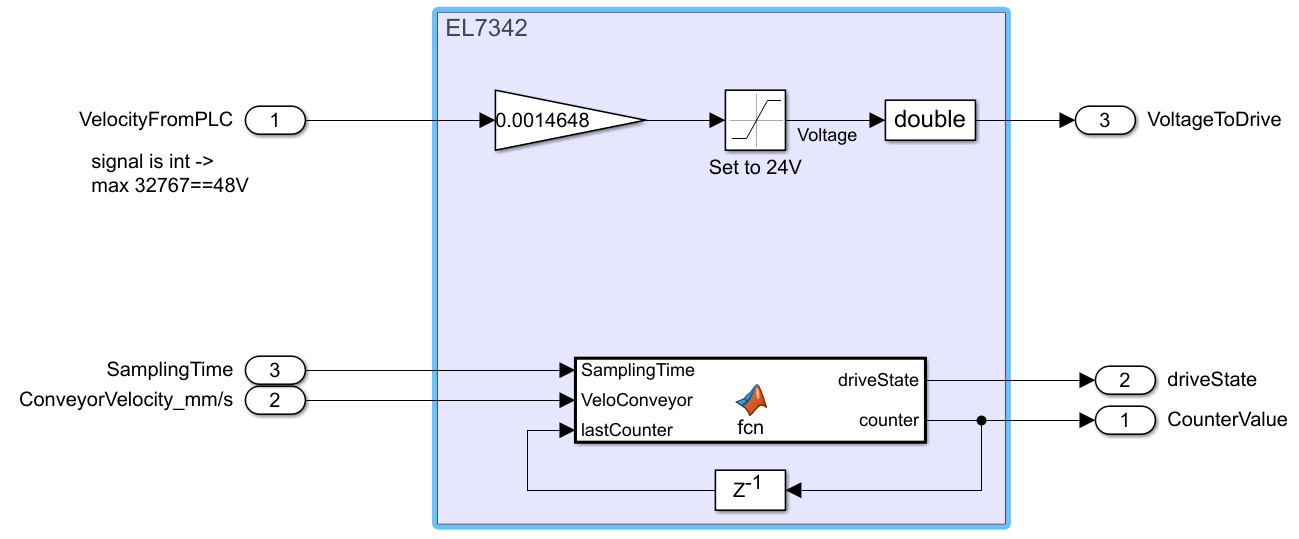
\includegraphics[width=.95\linewidth]{figures/ExampleConveyorModelKlemme.PNG}
%			\caption{Model of the used IO module}
%			\label{fig:ExampleFillingKlemmeModel}
%		\end{subfigure}
%		\caption{Use of the behaviour model in \textit{Simulink} for example \textit{conveyor belt}}
%		\label{fig:ExampleFillingUseModel}
%	\end{figure}
%    
%\subsubsection{PLC Code}
%    The code for the PLC remains very minimalistic in this example, as a result of the used NC axis. %This axis can be controlled via functions in the software, but in this case the graphical %interface is sufficient for simple commissioning and the first steps with the motor control. If %in the next step the software of the entire station with the additional components, such as the %dosing units with the stoppers and the sensors, should be created, the control of the motors in %own \textit{function blocks} is recommended. In these blocks, the NC axes are then controlled %via normal commands in the source code. \\ 
%    
%    % Kommunikation und Encoden und Verlinkung mit der Achse
%    Instead, the PLC software consists of compressing and decompressing the variables for %communication with the simulation. For this purpose, the current reference velocity must be %compressed and the actual position must be decompressed with the current state of the motor %terminal. These three variables are linked to the instance of the NC axis at the corresponding %places. The code for this example can be found in \autoref{lst:ConveyorbeltSolution} and with %this, the control of the motor can now be achieved by means of the graphical interface.
%  \lstinputlisting[basicstyle=\tiny, caption={Main program of example \textit{Conveyor Belt}}, %label=lst:ConveyorbeltSolution]{sourcecode/ExampleConveyorMainProgram.xml}
%
%
%
%\subsection{Module \textit{Cartesian Gripper}}
%\subsection{Module \textit{Load Cell}}
%\subsection{Module \textit{Thermal Processing}}
	
	
\subsection{Complete Factory - Combining the Modules}
    % CAD 
    For the mechanical planning of the plant, the individual modules are combined and positioned in an assembly. This process is a standard activity for an average user of \textit{Inventor}. \\
    
    % Hil Aufbau - Kommunikation
    As already mentioned in \autoref{sec:ExampleSetupTesting}, virtual commissioning takes place in a HIL system. Here, the PLC control and the behaviour models of the plant are executed on two different IPCs, which exchange the respective state via the real-time capable EAP interface. A publisher and subscriber are created on both IPCs and linked to the respective variables of the process image in order to establish communication. \\
    
    % Verhaltensmodell
    On the IPC with the simulation of the plant first a new \textit{TwinCAT} project is created and the \textit{TcCom} objects of the individual modules are instantiated. These objects are then assigned to a task with \SI{10}{\milli\second}. The outputs from this model are set as publish variables and the inputs as subscribe variables in the EAP communication. \\
    % PLC Code
    On the second IPC with the controlling software a new \textit{TwinCAT} project is also created and the clock time is set to \SI{10}{\milli\second}. In this project now the \textit{function blocks} of the individual modules are imported and called cyclically in the \textit{MAIN} program. Furthermore, in the \textit{MAIN} program the higher-level control between the modules is created and linked to the inputs and outputs of the \textit{function blocks}. \\
    For the used drives several NC axes must be added in \textit{TwinCAT} and parameterized with the corresponding settings from the individual data sheets. \\
    To establish EAP communication with the simulation of the plant, the outputs of the controller (actuators) are set as publish variables and the inputs (sensors) as subscribe variables. Afterwards, they are linked to the according variables in the process image. \\
    
    % Complete
    As soon as the two IPCs are configured, the runtime is started. From this point on, the plant is simulated on the first IPC and the control on the second IPC can be tested. Finally, a virtual commissioning can be performed with this setup.
    
	
%\section{Visualization \colorbox{orange}{Weg?}}
%    The current state of the PLC software and consequently the state of the plant is visualized in this example directly in the CAD software \textit{Inventor}. This implementation is done as a plugin in \textit{Inventor}, where the objective is a pure visualization of the state. The calculations and the user inputs are done directly in the PLC and in the defined task time. Thus the system as a whole remains real-time capable and, for example, controls can be implemented and tested under realistic conditions. \\
%    A disadvantage of this kind of implementation is the strongly limited frame rate of the graphic output in the range of about \SI{1}{\hertz} depending on the complexity of the assembly. This results from the required time for an update of the CAD model, which has to be done for every new value of of the PLC. Only in this way the current state is shown and not old values. However, this problem only affects the graphical output and has no influence on the control itself. To avoid this problem, \textit{Beckhoff} is currently developing a target for CAD software with the name \textit{TE1130} \cite{BeckhoffCadProduct}. With this target it should be possible to set the position of components in the software depending on a variable in the PLC and the update of the assembly will be optimized. As a result, a faster frame rate should be possible.  \\
    
%    The communication with the PLC is done via the \textit{ADS} protocol from \textit{Beckhoff}. In this communication the variables are read from the PLC and written as user parameters in \textit{Inventor}. The variables of the PLC contain the signals to and from the hardware. \\
%    If, for example, a piston is extended in the controller, which corresponds to setting a Boolean, the piston should also be extended in the CAD model. For this purpose, the relative position of the piston is linked to a user parameter in the CAD and set accordingly. \\

\ifundef{\WithVisualization}{}{
    \color{brown}
    \subsection{Visualization in \textit{Inventor}}
        As mentioned before, the current state of the PLC is shown directly in \textit{Inventor} in this example. Therefore the desired variables of the PLC are linked with the constraints in the CAD assembly according to the instruction \cite{BeckhoffCadAnleitung}. It should be noted here that in the current beta version of the used product only values of an NC axis can be exported from \textit{TwinCAT}. As a result, for each variable that should be read from \textit{TwinCAT}, an NC axis and a link between the actual value of the NC axis and the variable must be created. This finally makes the variable in \textit{Inventor} available. A screenshot from \textit{Inventor} with the shown state of the PLC can be found in \autoref{fig:VisuInInventor}.
        \begin{figure}[htp]
        	\centering
        	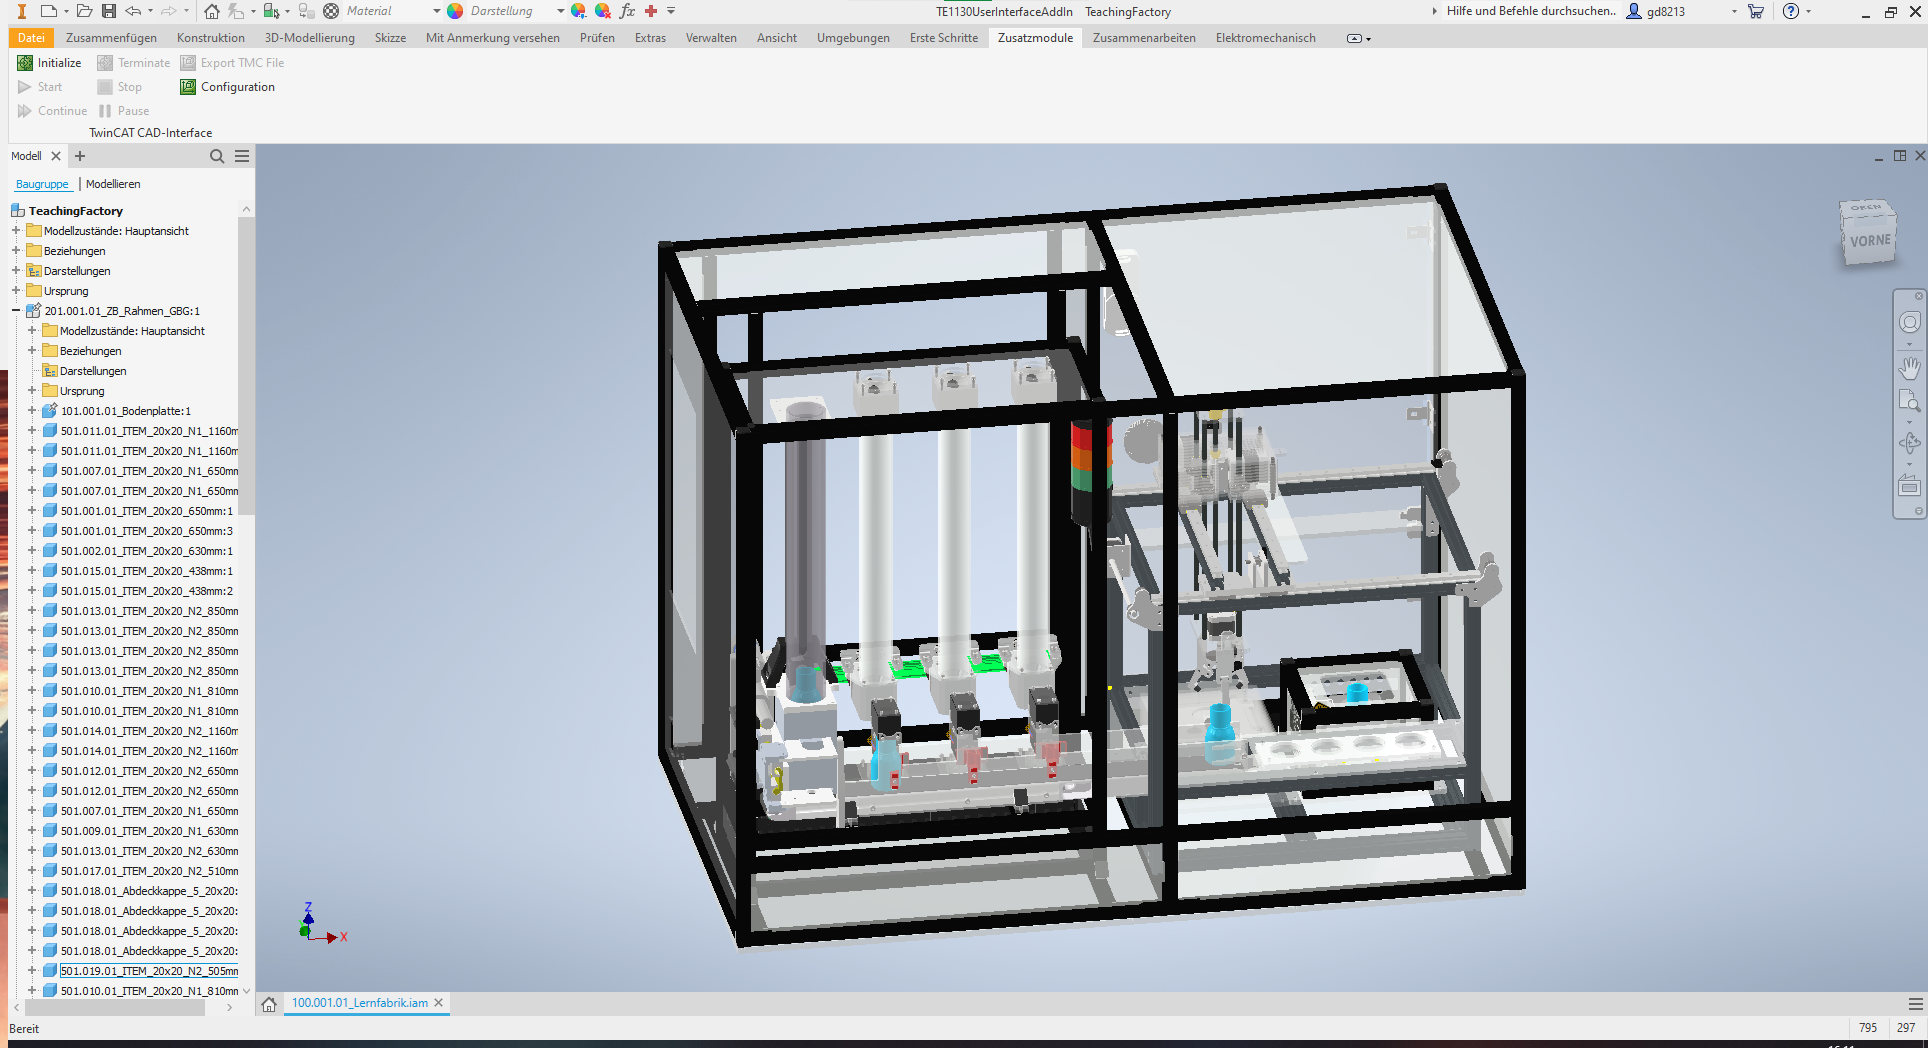
\includegraphics[width=0.9\linewidth]{figures/ScreenshotInventorVisu.png}
        	\caption[Screenshot of the visualization in \textit{Inventor}.]{Screenshot of the visualization in \textit{Inventor}, where the position of the pistons and the cartesian gripper is set from the PLC. }
        	\label{fig:VisuInInventor}
        \end{figure}
        
        \color{black}
}


\section{Summary}
    In this chapter, the proposed data structure is used in a real-life application and tested for its practical usability. An exemplary plant is divided into several modules and a data structure is created for each module and prepared for exchange. For this purpose, the CAD data with and without kinematics are exported, the behaviour model is created and the control code for the PLC is written. In the second step, this information is then imported from that data structure and integrated into a setup for a virtual commissioning. The simulation of the plant is executed in a second IPC in parallel with the control PLC, with the necessary communication taking place in real-time via EAP.\\
    

    %The first example deals with a \textit{separation}, where digital signals have to be read from three sensors and have to be written to two pistons. The CAD data with the kinematization is available in the native format of the software \textit{Inventor} where the customer uses the same software. For this reason, there is no need to recreate the kinematization on the customer's side. The behaviour model as \textit{.fmu} file describes the whole station and provides the sensor signals depending on the filling level of the input storage. The PLC code in \textit{PLCopen} format includes a \textit{function block} with a state machine in which the control logic is implemented. \\
   % Due to the formats of this data, the information can be integrated in the virtual commissioning without major effort and thus a setup for testing the plant is quickly available. The customer only has to write the main program of the PLC software and include there the provided \textit{function block} and create the simulation in \textit{Simulink} with the communication with the PLC. \\
    
    %The second example examines the virtual commissioning of a conveyor belt in more detail. This conveyor belt is driven by a DC motor, which also has an additional encoder on the motor axis. The PLC software now has to control the motor via a corresponding signal and process the feedback from the encoder. In contrast to the first example, the CAD data is available without kinematization in the neutral \textit{.step} format and, as a result, must be newly created by the customer. In the behaviour model, the DC motor is described in the form of a transfer function, with the voltage signal as input and the velocity on the conveyor belt as output. A PLC code is not supplied by the manufacturer and therefore has to be written by the customer. This data is again bundled in the data structure and sent to the customer.\\
    %Setting up the simulation for virtual commissioning and, as part of this, importing the data involves more effort for the customer in this example. First, the CAD assembly must be converted and newly kinematized. Then the model of the motor must be integrated in the simulation in \textit{Simulink} and additionally the motor terminal of the PLC must be modeled. Again, the communication with the PLC is part of the setup in the simulation. Finally, the virtual commissioning of the motor control is done via the graphical user interface in \textit{TwinCAT}.
    